\documentclass[11pt]{article}

\usepackage[margin=1in]{geometry}
\usepackage[T1]{fontenc}
\usepackage[utf8]{inputenc}
\usepackage{lmodern}
\usepackage{amsmath,amssymb,amsthm,mathtools}
\usepackage{enumitem}
\usepackage{hyperref}
\usepackage[most]{tcolorbox}
\usepackage{xcolor}
\usepackage{fancyhdr}
\usepackage{titlesec}
\usepackage{array}
\usepackage{longtable}
\usepackage{booktabs}
\usepackage{microtype}
\usepackage{tabularx}

\hypersetup{colorlinks=true, linkcolor=blue!60!black, urlcolor=blue!60!black, citecolor=blue!60!black}

\pagestyle{fancy}
\fancyhf{}
\lhead{DSC 190/291 Assignment 7}
\rhead{Dhruv Patel}
\cfoot{\thepage}

\titleformat{\section}{\large\bfseries}{\thesection.}{0.5em}{}
\titleformat{\subsection}{\normalsize\bfseries}{\thesubsection.}{0.5em}{}
\titleformat{\subsubsection}{\normalsize\itshape}{\thesubsubsection.}{0.5em}{}

\newtheorem{claim}{Claim}
\newtheorem{lemma}{Lemma}
\newtheorem{theorem}{Theorem}
\newtheorem{corollary}{Corollary}
\newtheorem{proposition}{Proposition}

\newcommand{\E}{\mathbb{E}}
\newcommand{\Pbb}{\mathbb{P}}
\newcommand{\R}{\mathbb{R}}
\newcommand{\N}{\mathbb{N}}
\newcommand{\calD}{\mathcal{D}}
\newcommand{\calH}{\mathcal{H}}
\newcommand{\calF}{\mathcal{F}}
\newcommand{\calG}{\mathcal{G}}
\newcommand{\calX}{\mathcal{X}}
\newcommand{\calY}{\mathcal{Y}}
\newcommand{\sign}{\mathrm{sign}}
\newcommand{\ind}{\mathbf{1}}
\newcommand{\eps}{\varepsilon}

\tcbset{
  colback=white,
  colframe=black!75,
  boxrule=0.8pt,
  arc=2pt,
  left=8pt,
  right=8pt,
  top=8pt,
  bottom=8pt
}

\newtcolorbox{solutionbox}{
    colback=white,
    colframe=black,
    boxrule=0.5pt,
    breakable
}

\title{\textbf{DSC 190/291 Assignment 7}\\Detailed Write-Up}
\author{Dhruv Patel}
\date{\today}

\begin{document}

\maketitle
\tableofcontents
\newpage

% =====================================================
\section{Kernel Methods}
% =====================================================
This homework continues the scale-sensitive complexity theme from Homework~6, 
where generalization is controlled by norms and margins rather than by dimension.

Let $\mathcal{U}$ be a Hilbert space with inner product $\langle \cdot,\cdot \rangle$ 
and induced norm $\|\cdot\|$, and let $\varphi : \mathcal{X} \to \mathcal{U}$ be 
a feature map with associated kernel 

\[
K(x,x') = \langle \varphi(x), \varphi(x') \rangle.
\]

For $B > 0$, let 

\[
\mathcal{H}_{K,B} 
= 
\{\, x \mapsto \langle w, \varphi(x) \rangle : w \in \mathcal{U},\ \|w\| \le B \,\}
\]
be the predictors of RKHS norm at most $B$.

For a sample $S = (x_1,\ldots,x_n)$ and a real-valued function class $\mathcal{F}$, 
write the empirical Rademacher complexity


\[
\widehat{\mathcal{R}}_{S}(\mathcal{F})
=
\mathbb{E}_{\sigma}
\sup_{f \in \mathcal{F}}
\frac{1}{n}
\sum_{i=1}^n \sigma_i f(x_i),
\]


where $\sigma_1,\ldots,\sigma_n$ are independent uniform signs.  
Write also


\[
\mathcal{R}_{\mathcal{D},n}(\mathcal{F})
=
\mathbb{E}_{S \sim \mathcal{D}^n}
\widehat{\mathcal{R}}_{S}(\mathcal{F}).
\]

\begin{enumerate}

\item \textbf{Norm-based kernel bound.}

Prove the empirical bound
\[
\widehat{\mathcal R}_S(\mathcal H_{K,B})
\le
\frac{B}{n}
\sqrt{\sum_{i=1}^n K(x_i,x_i)},
\]
and conclude the distribution-level bound
\[
\mathcal R_{\mathcal D^n}(\mathcal H_{K,B})
\le
B\sqrt{\frac{\E[K(X,X)]}{n}}.
\]

\begin{solutionbox}
\textbf{Goal.}

We want to derive an upper bound on the empirical Rademacher complexity of the RKHS ball
\[
\mathcal H_{K,B}
=
\left\{
x\mapsto \langle w,\varphi(x)\rangle :
\|w\|\le B
\right\},
\]
where the complexity bound depends only on the norm bound $B$ and the kernel diagonal terms
\[
K(x_i,x_i).
\]

The important idea is that although the feature space $\mathcal U$ may be extremely high-dimensional or even infinite-dimensional, the complexity of the class can still be controlled entirely through kernel evaluations.

\medskip

\textbf{Step 1: Start from the empirical Rademacher complexity definition.}

Recall that the empirical Rademacher complexity of a function class $\mathcal F$ on a sample
\[
S=(x_1,\ldots,x_n)
\]
is
\[
\widehat{\mathcal R}_S(\mathcal F)
=
\E_\sigma
\left[
\sup_{f\in\mathcal F}
\frac1n
\sum_{i=1}^n
\sigma_i f(x_i)
\right],
\]
where
\[
\sigma_1,\ldots,\sigma_n
\]
are independent Rademacher random variables taking values in $\{-1,+1\}$ uniformly.

For the RKHS ball $\mathcal H_{K,B}$,
every predictor has the form
\[
f_w(x)=\langle w,\varphi(x)\rangle
\]
with
\[
\|w\|\le B.
\]

Substituting this into the definition gives
\[
\widehat{\mathcal R}_S(\mathcal H_{K,B})
=
\E_\sigma
\sup_{\|w\|\le B}
\frac1n
\sum_{i=1}^n
\sigma_i
\langle w,\varphi(x_i)\rangle.
\]

Using linearity of the inner product, move $w$ outside the sum:
\[
=
\E_\sigma
\sup_{\|w\|\le B}
\frac1n
\left\langle
w,
\sum_{i=1}^n
\sigma_i\varphi(x_i)
\right\rangle.
\]

At this point, the entire optimization problem has been reduced to understanding the geometry of the random vector
\[
\sum_{i=1}^n\sigma_i\varphi(x_i)
\]
inside the Hilbert space.

\medskip

\textbf{Step 2: Apply the Cauchy--Schwarz inequality.}

For any vectors $u,v$ in a Hilbert space,
\[
\langle u,v\rangle
\le
\|u\|\,\|v\|.
\]

Applying this inequality with
\[
u=w,
\qquad
v=\sum_{i=1}^n\sigma_i\varphi(x_i),
\]
we obtain
\[
\left\langle
w,
\sum_{i=1}^n\sigma_i\varphi(x_i)
\right\rangle
\le
\|w\|
\left\|
\sum_{i=1}^n\sigma_i\varphi(x_i)
\right\|.
\]

Since the supremum is only over vectors satisfying
\[
\|w\|\le B,
\]
the largest possible value of the inner product is bounded by
\[
B
\left\|
\sum_{i=1}^n\sigma_i\varphi(x_i)
\right\|.
\]

Therefore,
\[
\widehat{\mathcal R}_S(\mathcal H_{K,B})
\le
\frac{B}{n}
\E_\sigma
\left\|
\sum_{i=1}^n\sigma_i\varphi(x_i)
\right\|.
\]

So far, we have reduced the problem to controlling the expected norm of a random signed combination of feature vectors.

\medskip

\textbf{Step 3: Use Jensen's inequality to simplify the expectation.}

The square-root function is concave, so Jensen's inequality implies
\[
\E[Z]
\le
\sqrt{\E[Z^2]}
\]
for any nonnegative random variable $Z$.

Apply this with
\[
Z=
\left\|
\sum_{i=1}^n\sigma_i\varphi(x_i)
\right\|.
\]

Then
\[
\E_\sigma
\left\|
\sum_{i=1}^n\sigma_i\varphi(x_i)
\right\|
\le
\sqrt{
\E_\sigma
\left\|
\sum_{i=1}^n\sigma_i\varphi(x_i)
\right\|^2
}.
\]

Substituting into the previous inequality gives
\[
\widehat{\mathcal R}_S(\mathcal H_{K,B})
\le
\frac{B}{n}
\sqrt{
\E_\sigma
\left\|
\sum_{i=1}^n\sigma_i\varphi(x_i)
\right\|^2
}.
\]

Now the remaining task is to compute this second moment exactly.

\medskip

\textbf{Step 4: Expand the squared norm.}

Using the Hilbert space identity
\[
\|v\|^2=\langle v,v\rangle,
\]
we expand:
\[
\left\|
\sum_{i=1}^n\sigma_i\varphi(x_i)
\right\|^2
=
\left\langle
\sum_{i=1}^n\sigma_i\varphi(x_i),
\sum_{j=1}^n\sigma_j\varphi(x_j)
\right\rangle.
\]

Using bilinearity of the inner product,
\[
=
\sum_{i=1}^n
\sum_{j=1}^n
\sigma_i\sigma_j
\langle
\varphi(x_i),
\varphi(x_j)
\rangle.
\]

Since
\[
\langle
\varphi(x_i),
\varphi(x_j)
\rangle
=
K(x_i,x_j),
\]
this becomes
\[
=
\sum_{i=1}^n
\sum_{j=1}^n
\sigma_i\sigma_j
K(x_i,x_j).
\]

Take expectation over the independent Rademacher signs.

For $i\neq j$,
\[
\E[\sigma_i\sigma_j]
=
\E[\sigma_i]\E[\sigma_j]
=
0,
\]
because each Rademacher variable has mean zero.

For diagonal terms,
\[
\E[\sigma_i^2]=1.
\]

Therefore every off-diagonal term vanishes, leaving only the diagonal contributions:
\[
\E_\sigma
\left\|
\sum_{i=1}^n\sigma_i\varphi(x_i)
\right\|^2
=
\sum_{i=1}^n
K(x_i,x_i).
\]

Substitute this back into the previous inequality:
\[
\widehat{\mathcal R}_S(\mathcal H_{K,B})
\le
\frac{B}{n}
\sqrt{
\sum_{i=1}^nK(x_i,x_i)
}.
\]

Thus we obtain the empirical bound
\[
\boxed{
\widehat{\mathcal R}_S(\mathcal H_{K,B})
\le
\frac{B}{n}
\sqrt{
\sum_{i=1}^nK(x_i,x_i)
}.
}
\]

\medskip

\textbf{Step 5: Derive the distribution-level bound.}

Now take expectation over random samples
\[
S\sim\mathcal D^n.
\]

By definition,
\[
\mathcal R_{\mathcal D^n}(\mathcal H_{K,B})
=
\E_S
\widehat{\mathcal R}_S(\mathcal H_{K,B}).
\]

Using the empirical bound,
\[
\mathcal R_{\mathcal D^n}(\mathcal H_{K,B})
\le
\E_S
\left[
\frac{B}{n}
\sqrt{
\sum_{i=1}^nK(x_i,x_i)
}
\right].
\]

Apply Jensen's inequality again:
\[
\E[\sqrt{Z}]
\le
\sqrt{\E[Z]}.
\]

Therefore,
\[
\mathcal R_{\mathcal D^n}(\mathcal H_{K,B})
\le
\frac{B}{n}
\sqrt{
\E_S
\sum_{i=1}^nK(x_i,x_i)
}.
\]

Since the examples are i.i.d.,
\[
\E_S
\sum_{i=1}^nK(x_i,x_i)
=
n\E[K(X,X)].
\]

Substituting gives
\[
\mathcal R_{\mathcal D^n}(\mathcal H_{K,B})
\le
\frac{B}{n}
\sqrt{
n\E[K(X,X)]
}.
\]

Simplifying,
\[
\boxed{
\mathcal R_{\mathcal D^n}(\mathcal H_{K,B})
\le
B
\sqrt{
\frac{\E[K(X,X)]}{n}
}.
}
\]

\medskip

\textbf{Interpretation.}

This result is important because it shows that the complexity of the RKHS hypothesis class depends on:
\begin{itemize}
    \item the norm constraint $B$,
    \item the average kernel diagonal magnitude,
    \item the sample size $n$,
\end{itemize}
but does \emph{not} explicitly depend on the ambient dimension of the feature space.

Even if the feature map $\\varphi(x)$ lives in an infinite-dimensional Hilbert space, the class can still have controlled complexity as long as the RKHS norm and kernel diagonal terms remain bounded.
\end{solutionbox}

\item \textbf{Representer theorem.}

The space $\mathcal{U}$ may be infinite \hyp dimensional, yet for any $\lambda > 0$ 
the regularized objective

\[
J(w) 
= 
\frac{1}{n} \sum_{i=1}^n 
\mathrm{loss}\!\left( \langle w, \varphi(x_i) \rangle ; y_i \right)
\;+\;
\lambda \|w\|^2
\]

can be minimized over finitely many coefficients. This is the representer theorem: 
prove that whenever $J$ attains a minimum over $w \in \mathcal{U}$, some minimizer has the form

\[
w^\ast = \sum_{j=1}^n \alpha_j \varphi(x_j), 
\qquad 
\alpha \in \mathbb{R}^n.
\]

Then rewrite $J$ as a minimization over $\alpha \in \mathbb{R}^n$ in which the data enter 
only through the Gram matrix $K_S$, with entries
\[
(K_S)_{ij} = K(x_i, x_j).
\]

\begin{solutionbox}

\textbf{Goal.}

We want to prove the representer theorem. The key statement is that even though the Hilbert space
\[
\mathcal U
\]
may be infinite-dimensional, the optimization problem
\[
J(w)
=
\frac1n
\sum_{i=1}^n
\mathrm{loss}(\langle w,\varphi(x_i)\rangle;y_i)
+
\lambda\|w\|^2
\]
can always be solved using only finitely many parameters.

More specifically, we will show that some minimizer always lies inside the span of the training feature vectors
\[
\varphi(x_1),\ldots,\varphi(x_n).
\]

This is one of the most important structural results in kernel methods because it reduces an optimization problem in a potentially infinite-dimensional space to a finite-dimensional optimization problem involving only the Gram matrix.

\medskip

\textbf{Step 1: Define the training span.}

Consider the subspace generated by the feature vectors of the training data:
\[
V
=
\mathrm{span}
\{
\varphi(x_1),
\varphi(x_2),
\ldots,
\varphi(x_n)
\}.
\]

Since this span is generated by only $n$ vectors, it is finite-dimensional even if the ambient Hilbert space $\mathcal U$ is infinite-dimensional.

Now take any vector
\[
w\in\mathcal U.
\]

Because $\mathcal U$ is a Hilbert space, every vector admits an orthogonal decomposition relative to the subspace $V$:
\[
w=w_{\parallel}+w_{\perp},
\]
where
\[
w_{\parallel}\in V,
\qquad
w_{\perp}\perp V.
\]

Geometrically:
\begin{itemize}
    \item $w_{\parallel}$ is the projection of $w$ onto the training span,
    \item $w_{\perp}$ is the component orthogonal to every training feature vector.
\end{itemize}

The entire proof revolves around understanding how these two components affect the objective function.

\medskip

\textbf{Step 2: Show that predictions depend only on the projection.}

The loss term depends on the predictions
\[
\langle w,\varphi(x_i)\rangle.
\]

Substitute the orthogonal decomposition:
\[
\langle w,\varphi(x_i)\rangle
=
\langle
w_{\parallel}+w_{\perp},
\varphi(x_i)
\rangle.
\]

Using linearity of the inner product,
\[
=
\langle w_{\parallel},\varphi(x_i)\rangle
+
\langle w_{\perp},\varphi(x_i)\rangle.
\]

Now observe an important fact:
\[
\varphi(x_i)\in V
\]
for every training point.

Since
\[
w_{\perp}\perp V,
\]
it follows that
\[
\langle w_{\perp},\varphi(x_i)\rangle=0.
\]

Therefore,
\[
\langle w,\varphi(x_i)\rangle
=
\langle w_{\parallel},\varphi(x_i)\rangle.
\]

This means the predictions on the training data are completely determined by the projected component
\[
w_{\parallel}.
\]

The orthogonal component
\[
w_{\perp}
\]
has absolutely no effect on the empirical loss term.

Consequently,
\[
\frac1n
\sum_{i=1}^n
\mathrm{loss}(\langle w,\varphi(x_i)\rangle;y_i)
=
\frac1n
\sum_{i=1}^n
\mathrm{loss}(\langle w_{\parallel},\varphi(x_i)\rangle;y_i).
\]

Thus the loss depends only on the projection onto the training span.

\medskip

\textbf{Step 3: Compare the regularization terms.}

Next analyze the norm term.

Because
\[
w_{\parallel}\perp w_{\perp},
\]
the Pythagorean theorem in Hilbert spaces gives
\[
\|w\|^2
=
\|w_{\parallel}\|^2
+
\|w_{\perp}\|^2.
\]

Since
\[
\|w_{\perp}\|^2\ge0,
\]
we immediately obtain
\[
\|w\|^2
\ge
\|w_{\parallel}\|^2.
\]

Now compare the full objectives.

The empirical loss terms are identical:
\[
\mathrm{loss}(w)=\mathrm{loss}(w_{\parallel}).
\]

But the regularization term satisfies
\[
\lambda\|w\|^2
=
\lambda\|w_{\parallel}\|^2
+
\lambda\|w_{\perp}\|^2.
\]

Since
\[
\lambda>0,
\]
any nonzero orthogonal component strictly increases the objective.

Therefore,
\[
J(w)
=
J(w_{\parallel})
+
\lambda\|w_{\perp}\|^2
\ge
J(w_{\parallel}).
\]

Hence removing the orthogonal component can never increase the objective and usually decreases it.

This proves that some minimizer must satisfy
\[
w_{\perp}=0.
\]

Therefore every minimizer lies entirely inside the training span:
\[
w^*\in V.
\]

Since $V$ is spanned by the training feature vectors,
\[
\boxed{
w^*
=
\sum_{j=1}^n
\alpha_j\varphi(x_j)
}
\]
for some coefficients
\[
\alpha_1,\ldots,\alpha_n\in\R.
\]

This is exactly the representer theorem.

\medskip

\textbf{Step 4: Rewrite predictions using the kernel.}

Now substitute the representation
\[
w
=
\sum_{j=1}^n
\alpha_j\varphi(x_j).
\]

For a training example $x_i$,
\[
\langle w,\varphi(x_i)\rangle
=
\left\langle
\sum_{j=1}^n
\alpha_j\varphi(x_j),
\varphi(x_i)
\right\rangle.
\]

Using linearity,
\[
=
\sum_{j=1}^n
\alpha_j
\langle
\varphi(x_j),
\varphi(x_i)
\rangle.
\]

By the kernel definition,
\[
K(x_j,x_i)
=
\langle
\varphi(x_j),
\varphi(x_i)
\rangle.
\]

Therefore,
\[
\langle w,\varphi(x_i)\rangle
=
\sum_{j=1}^n
\alpha_jK(x_j,x_i).
\]

Define the Gram matrix
\[
K_S\in\R^{n\times n}
\]
by
\[
(K_S)_{ij}
=
K(x_i,x_j).
\]

Then the vector of predictions on the training sample can be written compactly as
\[
K_S\alpha.
\]

Thus all predictions are determined entirely by kernel evaluations between training points.

\medskip

\textbf{Step 5: Rewrite the norm term.}

Now compute the RKHS norm.

Using the representation of $w$,
\[
\|w\|^2
=
\langle w,w\rangle.
\]

Substitute the expansion:
\[
=
\left\langle
\sum_i\alpha_i\varphi(x_i),
\sum_j\alpha_j\varphi(x_j)
\right\rangle.
\]

Expand using bilinearity:
\[
=
\sum_i\sum_j
\alpha_i\alpha_j
\langle
\varphi(x_i),
\varphi(x_j)
\rangle.
\]

Again replace the inner products with kernel evaluations:
\[
=
\sum_i\sum_j
\alpha_i\alpha_j
K(x_i,x_j).
\]

In matrix form,
\[
\boxed{
\|w\|^2
=
\alpha^\top K_S\alpha.
}
\]

\medskip

\textbf{Step 6: Final finite-dimensional optimization problem.}

Substituting the prediction formula and norm formula into the original objective yields
\[
J(\alpha)
=
\frac1n
\sum_{i=1}^n
\mathrm{loss}((K_S\alpha)_i;y_i)
+
\lambda\alpha^\top K_S\alpha.
\]

Therefore the optimization problem becomes
\[
\boxed{
\min_{\alpha\in\R^n}
\frac1n
\sum_{i=1}^n
\mathrm{loss}((K_S\alpha)_i;y_i)
+
\lambda\alpha^\top K_S\alpha.
}
\]

\medskip

\textbf{Interpretation.}

This result is fundamental because it shows that kernel learning never requires explicitly optimizing over the infinite-dimensional feature space.

Instead:
\begin{itemize}
    \item all predictors can be represented using only training examples,
    \item optimization reduces to $n$ coefficients,
    \item the feature map appears only through kernel evaluations,
    \item the entire learning problem is encoded by the Gram matrix.
\end{itemize}

This is the reason kernel methods remain computationally tractable even when the underlying feature space is infinite-dimensional.

\end{solutionbox}

\end{enumerate}

% =====================================================
\section{$\ell_1$ Rademacher Complexity}
% =====================================================
Throughout this part, $\widehat{\mathcal{R}}_{S}$ denotes the empirical Rademacher 
complexity defined in Part~A.
\begin{enumerate}

\item \textbf{Convex hulls.}

Let $\mathcal F$ be a finite class of real-valued functions. Its convex hull is
\[
\operatorname{conv}(\mathcal F)
=
\left\{
\sum_{f\in\mathcal F}a_ff:
a_f\ge0,
\sum_fa_f=1
\right\}.
\]

Prove that empirical Rademacher complexity is unchanged by taking the conves hull:
\[
\widehat{\mathcal R}_S(\operatorname{conv}(\mathcal F))
=
\widehat{\mathcal R}_S(\mathcal F).
\]

\begin{solutionbox}

\textbf{Goal.}

We want to prove that taking convex combinations of functions does not increase empirical Rademacher complexity.

More precisely, if
\[
\operatorname{conv}(\mathcal F)
\]
denotes the convex hull of a finite function class $\mathcal F$, then we want to show
\[
\widehat{\mathcal R}_S(\operatorname{conv}(\mathcal F))
=
\widehat{\mathcal R}_S(\mathcal F).
\]

Intuitively, this result says that averaging functions together does not create additional complexity from the perspective of Rademacher averages. The ``most difficult'' function in the convex hull is always one of the original extreme points of the class.

\medskip

\textbf{Step 1: Recall the definition of empirical Rademacher complexity.}

For a function class $\mathcal F$ and sample
\[
S=(x_1,\ldots,x_n),
\]
the empirical Rademacher complexity is defined as
\[
\widehat{\mathcal R}_S(\mathcal F)
=
\E_\sigma
\left[
\sup_{f\in\mathcal F}
\frac1n
\sum_{i=1}^n
\sigma_if(x_i)
\right],
\]
where
\[
\sigma_1,\ldots,\sigma_n
\]
are independent Rademacher random variables taking values in
\[
\{-1,+1\}.
\]

The quantity
\[
\frac1n\sum_i\sigma_if(x_i)
\]
measures how well the function $f$ correlates with random noise on the sample.

The Rademacher complexity then measures the largest possible correlation achievable by functions in the class.

\medskip

\textbf{Step 2: Write down the convex hull definition.}

The convex hull of $\mathcal F$ is
\[
\operatorname{conv}(\mathcal F)
=
\left\{
\sum_{f\in\mathcal F}a_ff
:
a_f\ge0,
\quad
\sum_fa_f=1
\right\}.
\]

Thus every function
\[
h\in\operatorname{conv}(\mathcal F)
\]
is a convex combination of functions from $\mathcal F$.

The coefficients
\[
a_f
\]
behave like probabilities:
\begin{itemize}
    \item they are nonnegative,
    \item they sum to one.
\end{itemize}

Geometrically, the convex hull contains all weighted averages of functions from the original class.

\medskip

\textbf{Step 3: Start from the Rademacher complexity of the convex hull.}

By definition,
\[
\widehat{\mathcal R}_S(\operatorname{conv}(\mathcal F))
=
\E_\sigma
\left[
\sup_{h\in\operatorname{conv}(\mathcal F)}
\frac1n
\sum_{i=1}^n
\sigma_ih(x_i)
\right].
\]

Now let
\[
h=\sum_{f\in\mathcal F}a_ff
\]
be an arbitrary element of the convex hull.

Substitute this representation into the Rademacher expression:
\[
\frac1n
\sum_{i=1}^n
\sigma_ih(x_i)
=
\frac1n
\sum_{i=1}^n
\sigma_i
\left(
\sum_{f\in\mathcal F}a_ff(x_i)
\right).
\]

Using linearity of summation, interchange the sums:
\[
=
\sum_{f\in\mathcal F}
a_f
\left(
\frac1n
\sum_{i=1}^n
\sigma_if(x_i)
\right).
\]

Define
\[
c_f
=
\frac1n
\sum_{i=1}^n
\sigma_if(x_i).
\]

Then the expression becomes
\[
\sum_{f\in\mathcal F}a_fc_f.
\]

Thus the Rademacher quantity for a convex combination is itself a convex combination of the individual Rademacher quantities.

\medskip

\textbf{Step 4: Analyze the convex combination.}

The coefficients
\[
a_f
\]
form a convex combination, so
\[
\sum_{f\in\mathcal F}a_fc_f
\]
is a weighted average of the numbers
\[
c_f.
\]

A weighted average can never exceed the maximum value being averaged.

Therefore,
\[
\sum_{f\in\mathcal F}a_fc_f
\le
\max_{f\in\mathcal F}c_f.
\]

Equivalently,
\[
\sum_{f\in\mathcal F}
a_f
\left(
\frac1n
\sum_{i=1}^n
\sigma_if(x_i)
\right)
\le
\sup_{f\in\mathcal F}
\frac1n
\sum_{i=1}^n
\sigma_if(x_i).
\]

Since this holds for every convex combination,
\[
\sup_{h\in\operatorname{conv}(\mathcal F)}
\frac1n
\sum_{i=1}^n
\sigma_ih(x_i)
\le
\sup_{f\in\mathcal F}
\frac1n
\sum_{i=1}^n
\sigma_if(x_i).
\]

\medskip

\textbf{Step 5: Show equality holds.}

Now we prove the reverse inequality.

Observe that every function
\[
f\in\mathcal F
\]
already belongs to the convex hull.

Indeed, choose coefficients
\[
a_f=1,
\qquad
a_g=0
\quad
(g\neq f).
\]

Thus,
\[
\mathcal F
\subseteq
\operatorname{conv}(\mathcal F).
\]

Therefore,
\[
\sup_{f\in\mathcal F}
\frac1n
\sum_{i=1}^n
\sigma_if(x_i)
\le
\sup_{h\in\operatorname{conv}(\mathcal F)}
\frac1n
\sum_{i=1}^n
\sigma_ih(x_i).
\]

Combining both inequalities yields
\[
\sup_{h\in\operatorname{conv}(\mathcal F)}
\frac1n
\sum_{i=1}^n
\sigma_ih(x_i)
=
\sup_{f\in\mathcal F}
\frac1n
\sum_{i=1}^n
\sigma_if(x_i).
\]

Finally, taking expectation over the Rademacher signs gives
\[
\boxed{
\widehat{\mathcal R}_S(\operatorname{conv}(\mathcal F))
=
\widehat{\mathcal R}_S(\mathcal F).
}
\]

\medskip

\textbf{Interpretation.}

This result is extremely important in learning theory because it shows that convexification does not increase Rademacher complexity.

In other words:
\begin{itemize}
    \item adding mixtures or averages of predictors does not create additional complexity,
    \item the extreme points of the class already determine the complexity,
    \item linear optimization over a convex hull always achieves its optimum at an extreme point.
\end{itemize}

This fact is one of the core reasons why boosting and convex aggregation methods remain analyzable using the complexity of the underlying base class.

\medskip

\textbf{Lean formalization artifact.}

A supporting Lean 4 formalization for this convex-hull identity is included in
\[
\texttt{src/lean/Assignment7\_B1\_ConvexHull.lean}.
\]

\end{solutionbox}

\item \textbf{$\ell_1$ linear predictors.}

Let $\varphi:\mathcal X\to\R^d$ satisfy
\[
\|\varphi(x)\|_\infty\le R
\]
for all $x$, and define
\[
\mathcal H_B^1
=
\{x\mapsto \langle w,\varphi(x)\rangle : \|w\|_1\le B\}.
\]

Derive a logarithmic-in-dimension Rademacher bound for $\mathcal H_B^1$, Massart's finite-class lemma bounds the Rademacher complexity of a finite class; the convex-hull indetity from teh  previous problem is what connects $\mathcal H_B^1$ to such a class. 

\begin{solutionbox}

\textbf{Goal.}

We want to prove that the empirical Rademacher complexity of the $\\ell_1$ ball grows only logarithmically with the ambient dimension $d$.

More precisely, for the hypothesis class
\[
\mathcal H_B^1
=
\left\{
x\mapsto \langle w,\varphi(x)\rangle :
\|w\|_1\le B
\right\},
\]
where the feature map satisfies
\[
\|\varphi(x)\|_\infty\le R,
\]
we want to show
\[
\widehat{\mathcal R}_S(\mathcal H_B^1)
\le
BR
\sqrt{
\frac{2\log(2d)}{n}
}.
\]

The key idea is that the $\\ell_1$ ball behaves like the convex hull of the coordinate functions. Once we rewrite the class in this form, we can combine:
\begin{itemize}
    \item the convex-hull identity from Part B.1,
    \item Massart's finite-class lemma.
\end{itemize}

This produces a bound that depends only logarithmically on dimension rather than polynomially.

\medskip

\textbf{Step 1: Expand the linear predictor coordinate-wise.}

Take any predictor from the class
\[
\mathcal H_B^1.
\]

By definition, every function has the form
\[
f_w(x)
=
\langle w,\varphi(x)\rangle,
\]
where
\[
w=(w_1,\ldots,w_d)\in\R^d
\]
satisfies
\[
\|w\|_1
=
\sum_{j=1}^d|w_j|
\le B.
\]

Write the feature map coordinate-wise as
\[
\varphi(x)
=
(\varphi_1(x),\ldots,\varphi_d(x)).
\]

Then the predictor becomes
\[
f_w(x)
=
\sum_{j=1}^d
w_j\varphi_j(x).
\]

Thus every predictor is a linear combination of the coordinate functions
\[
\varphi_1,\ldots,\varphi_d.
\]

\medskip

\textbf{Step 2: Introduce the finite base class.}

Define the finite class
\[
\mathcal F
=
\{
\pm\varphi_j :
j=1,\ldots,d
\}.
\]

Explicitly,
\[
\mathcal F
=
\{
\varphi_1,\ldots,\varphi_d,
-\varphi_1,\ldots,-\varphi_d
\}.
\]

Therefore,
\[
|\mathcal F|=2d.
\]

The reason we include both signs is that the coefficients
\[
w_j
\]
may be positive or negative.

\medskip

\textbf{Step 3: Rewrite the $\\ell_1$ ball as a convex hull.}

We now show that every predictor in the $\\ell_1$ ball can be represented as a scaled convex combination of functions from $\\mathcal F$.

Take any
\[
w\in\R^d
\]
satisfying
\[
\|w\|_1\le B.
\]

Define
\[
a_j=\frac{|w_j|}{B}.
\]

Since
\[
\sum_{j=1}^d|w_j|
\le B,
\]
we obtain
\[
\sum_{j=1}^da_j
=
\frac1B\sum_{j=1}^d|w_j|
\le1.
\]

Now define the sign function
\[
s_j=\operatorname{sign}(w_j)\in\{-1,+1\}.
\]

Then
\[
w_j
=
Bs_ja_j.
\]

Substitute this into the predictor:
\[
f_w(x)
=
\sum_{j=1}^d
Bs_ja_j\varphi_j(x).
\]

Factor out $B$:
\[
=
B
\sum_{j=1}^d
a_j(s_j\varphi_j(x)).
\]

Each function
\[
s_j\varphi_j
\]
belongs to the class
\[
\mathcal F.
\]

Thus the predictor is a scaled convex combination of functions from $\\mathcal F$.

Consequently,
\[
\boxed{
\mathcal H_B^1
\subseteq
B\cdot\operatorname{conv}(\mathcal F).
}
\]

This is the key geometric step in the proof.

\medskip

\textbf{Step 4: Apply the convex-hull identity.}

From Part B.1, we proved that taking convex hulls does not change empirical Rademacher complexity:
\[
\widehat{\mathcal R}_S(\operatorname{conv}(\mathcal F))
=
\widehat{\mathcal R}_S(\mathcal F).
\]

Also, scaling a function class by a constant scales the Rademacher complexity by the same constant:
\[
\widehat{\mathcal R}_S(B\mathcal F)
=
B\widehat{\mathcal R}_S(\mathcal F).
\]

Since
\[
\mathcal H_B^1
\subseteq
B\cdot\operatorname{conv}(\mathcal F),
\]
monotonicity of Rademacher complexity gives
\[
\widehat{\mathcal R}_S(\mathcal H_B^1)
\le
\widehat{\mathcal R}_S(B\operatorname{conv}(\mathcal F)).
\]

Using the scaling property and convex-hull identity,
\[
=
B
\widehat{\mathcal R}_S(\operatorname{conv}(\mathcal F))
=
B
\widehat{\mathcal R}_S(\mathcal F).
\]

Therefore,
\[
\boxed{
\widehat{\mathcal R}_S(\mathcal H_B^1)
\le
B\widehat{\mathcal R}_S(\mathcal F).
}
\]

So the problem has now been reduced to bounding the complexity of a finite class.

\medskip

\textbf{Step 5: Apply Massart's finite-class lemma.}

We are given that
\[
\|\varphi(x)\|_\infty\le R.
\]

This means that every coordinate satisfies
\[
|\varphi_j(x)|\le R.
\]

Since the functions in
\[
\mathcal F
\]
are exactly the signed coordinate functions,
every function
\[
f\in\mathcal F
\]
satisfies
\[
|f(x)|\le R
\]
for all examples.

Massart's finite-class lemma states that if:
\begin{itemize}
    \item $|\mathcal F|<\infty$,
    \item every function is bounded in magnitude by $R$,
\end{itemize}
then
\[
\widehat{\mathcal R}_S(\mathcal F)
\le
R
\sqrt{
\frac{2\log|\mathcal F|}{n}
}.
\]

Since
\[
|\mathcal F|=2d,
\]
we obtain
\[
\widehat{\mathcal R}_S(\mathcal F)
\le
R
\sqrt{
\frac{2\log(2d)}{n}
}.
\]

Substituting into the previous inequality gives
\[
\widehat{\mathcal R}_S(\mathcal H_B^1)
\le
B
\left(
R
\sqrt{
\frac{2\log(2d)}{n}
}
\right).
\]

Therefore,
\[
\boxed{
\widehat{\mathcal R}_S(\mathcal H_B^1)
\le
BR
\sqrt{
\frac{2\log(2d)}{n}
}.
}
\]

\medskip

\textbf{Interpretation.}

This bound is extremely important because it shows that the complexity of the $\\ell_1$ ball depends only logarithmically on dimension.

In many high-dimensional learning problems:
\begin{itemize}
    \item the ambient dimension $d$ may be extremely large,
    \item sparse or approximately sparse predictors are still learnable,
    \item controlling the $\\ell_1$ norm is enough to control generalization.
\end{itemize}

The logarithmic dependence
\[
\log d
\]
is dramatically smaller than polynomial dependence on $d$.

This is one of the main theoretical reasons why:
\begin{itemize}
    \item sparse learning,
    \item Lasso-type methods,
    \item boosting methods,
    \item high-dimensional linear prediction
\end{itemize}
can generalize effectively even when
\[
d\gg n.
\]

\end{solutionbox}

\item \textbf{Comparison with sparsity bounds.}

In Homework~4 you showed that the class of $k$-sparse linear classifiers in 
$\mathbb{R}^d$ has VC dimension 


\[
O\!\left(k \log\!\left(\frac{e d}{k}\right)\right).
\]


With the VC generalization bound, with probability at least $1 - \delta$ over the draw 
of $S \sim \mathcal{D}^n$, every $k$-sparse linear classifier $h$ satisfies


\[
L^{0/1}_{\mathcal{D}}(h) - L^{0/1}_{S}(h)
\;\le\;
C \sqrt{\frac{k \log(e d / k) + \log(1/\delta)}{n}},
\]


for a universal constant $C$.  
Structural risk minimization makes the bound adapt to the unknown sparsity level $k$.

Using your Rademacher bound from the previous problem and the Week~7 uniform 
convergence theorem, derive the analogous bound for $\mathcal{H}^{1}_{B}$: a bound on


\[
L^{\ell}_{\mathcal{D}}(w) - L^{\ell}_{S}(w),
\]


holding with probability at least $1 - \delta$ over the draw of $S \sim \mathcal{D}^n$, 
uniformly over $\|w\|_{1} \le B$, for a fixed loss $\ell$ that is $G$-Lipschitz in the 
prediction and bounded in $[0,1]$.

These two bounds control different loss functionals, so they are not interchangeable 
guarantees. Compare them: which quantity is the complexity in each and which one is 
scale-sensitive; what extra step the $\ell_1$ bound needs before it can say anything 
about $0/1$ error; and exhibit a predictor for which the sparsity bound is vacuous 
while the $\ell_1$ bound is not.

\begin{solutionbox}

\textbf{Goal.}

We want to derive a uniform convergence bound for the hypothesis class
\[
\mathcal H_B^1
=
\left\{
x\mapsto\langle w,\varphi(x)\rangle :
\|w\|_1\le B
\right\}
\]
using the Rademacher complexity result from Part B.2.

After deriving the bound, we will compare it to sparsity-based VC dimension bounds and explain the conceptual difference between:
\begin{itemize}
    \item combinatorial sparsity control,
    \item scale-sensitive norm control.
\end{itemize}

The key point is that $\\ell_1$ complexity bounds can remain meaningful even when the predictor is dense, provided the total $\\ell_1$ norm remains small.

\medskip

\textbf{Step 1: Recall the Rademacher uniform convergence theorem.}

Let
\[
\ell(\hat y,y)
\]
be a loss function satisfying:
\begin{itemize}
    \item the loss is bounded in $[0,1]$,
    \item the loss is $G$-Lipschitz with respect to the prediction argument.
\end{itemize}

For a predictor $f$, define:
\[
L_{\mathcal D}^\ell(f)
=
\E_{(x,y)\sim\mathcal D}
[\ell(f(x),y)]
\]
as the population loss, and
\[
L_S^\ell(f)
=
\frac1n
\sum_{i=1}^n
\ell(f(x_i),y_i)
\]
as the empirical loss.

The Rademacher uniform convergence theorem from Week 7 states that with probability at least
\[
1-\delta,
\]
simultaneously for all predictors in the class,
\[
L_{\mathcal D}^\ell(f)
-
L_S^\ell(f)
\le
2G
\widehat{\mathcal R}_S(\mathcal H)
+
\sqrt{
\frac{\log(1/\delta)}{2n}
}.
\]

The theorem separates the generalization gap into two components:
\begin{enumerate}
    \item a complexity term involving the Rademacher complexity,
    \item a concentration term involving confidence parameter $\\delta$.
\end{enumerate}

We now apply this theorem to the $\\ell_1$ hypothesis class.

\medskip

\textbf{Step 2: Substitute the $\\ell_1$ Rademacher complexity bound.}

From Part B.2, we proved that
\[
\widehat{\mathcal R}_S(\mathcal H_B^1)
\le
BR
\sqrt{
\frac{2\log(2d)}{n}
}.
\]

Substitute this bound into the uniform convergence theorem:
\[
L_{\mathcal D}^\ell(w)
-
L_S^\ell(w)
\le
2G
\left(
BR
\sqrt{
\frac{2\log(2d)}{n}
}
\right)
+
\sqrt{
\frac{\log(1/\delta)}{2n}
}.
\]

Simplifying gives
\[
\boxed{
L_{\mathcal D}^\ell(w)
-
L_S^\ell(w)
\le
2GBR
\sqrt{
\frac{2\log(2d)}{n}
}
+
\sqrt{
\frac{\log(1/\delta)}{2n}
}.
}
\]

This bound holds uniformly over all predictors satisfying
\[
\|w\|_1\le B.
\]

\medskip

\textbf{Step 3: Interpret the bound.}

The dominant complexity term is
\[
BR
\sqrt{
\frac{\log d}{n}
}.
\]

Notice several important features:
\begin{itemize}
    \item dependence on dimension is only logarithmic,
    \item dependence on sample size is $1/\sqrt n$,
    \item dependence on the hypothesis class is controlled through the norm bound $B$.
\end{itemize}

This is fundamentally different from classical VC-style sparsity bounds.

\medskip

\textbf{Step 4: Compare with sparsity-based VC bounds.}

For sparse linear predictors with support size
\[
k=\|w\|_0,
\]
the VC-dimension-style bound typically depends on
\[
k\log\left(\frac{ed}{k}\right).
\]

This type of bound measures combinatorial complexity:
\begin{itemize}
    \item how many coordinates may be active,
    \item how many support patterns are possible,
    \item how many distinct classifiers can be realized.
\end{itemize}

In contrast, the $\\ell_1$ Rademacher bound measures scale-sensitive complexity.

Instead of counting active coordinates, it measures:
\begin{itemize}
    \item how large the coefficients are,
    \item how spread-out the predictor mass is,
    \item how large the overall $\\ell_1$ norm becomes.
\end{itemize}

Thus:
\[
\text{sparsity bound}
\quad\Longrightarrow\quad
\text{combinatorial control},
\]
whereas
\[
\ell_1\text{ bound}
\quad\Longrightarrow\quad
\text{scale-sensitive control}.
\]

\medskip

\textbf{Step 5: Example where the $\\ell_1$ bound is much stronger.}

Consider the dense predictor
\[
w
=
\left(
\frac1d,
\frac1d,
\ldots,
\frac1d
\right).
\]

This predictor uses every coordinate.

Therefore,
\[
\|w\|_0=d.
\]

If
\[
d\gg n,
\]
the sparsity-based VC bound becomes extremely large because the effective support size equals the full ambient dimension.

For example, the sparsity complexity term behaves roughly like
\[
\sqrt{
\frac{
d\log(ed/d)
}{n}
}
=
\sqrt{
\frac{d}{n}
}.
\]

This becomes vacuous when
\[
d
\]
is much larger than
\[
n.
\]

However, the $\\ell_1$ norm of this predictor is
\[
\|w\|_1
=
d\cdot\frac1d
=
1.
\]

Thus the $\\ell_1$ complexity bound becomes
\[
O\left(
\sqrt{
\frac{\log d}{n}
}
\right),
\]
which can remain small even for extremely large dimensions.

This demonstrates the central advantage of norm-based analysis:
\begin{itemize}
    \item predictors may be dense,
    \item ambient dimension may be huge,
    \item generalization can still occur if the overall norm is controlled.
\end{itemize}

\medskip

\textbf{Conceptual interpretation.}

The sparsity viewpoint asks:
\[
\text{``How many coordinates are used?''}
\]

The $\\ell_1$ viewpoint instead asks:
\[
\text{``How much total weight is used?''}
\]

These are fundamentally different notions of complexity.

The $\\ell_1$ framework is often much more flexible because it allows:
\begin{itemize}
    \item approximate sparsity,
    \item soft feature selection,
    \item distributed weights across many coordinates.
\end{itemize}

This is one of the main reasons why:
\begin{itemize}
    \item Lasso,
    \item boosting,
    \item sparse regularization methods,
    \item compressed sensing techniques
\end{itemize}
are analyzable using norm-based complexity bounds.

\end{solutionbox}

\end{enumerate}

% =====================================================
\section{Normalized $\ell_1$ Margins and FixedBoost}
% =====================================================
In this part the sample is $S = \bigl((x_1,y_1),\ldots,(x_n,y_n)\bigr)$ with labels $y_i \in \{-1,+1\}$, and $\mathcal{G}$ is a finite base class of binary 
predictors $g : \mathcal{X} \to \{-1,+1\}$, symmetric in the sense that 
$-g \in \mathcal{G}$ whenever $g \in \mathcal{G}$. A coefficient vector $w = (w_g)_{g \in \mathcal{G}}$ parameterizes the real-valued 
predictor $f_w(x) = \sum_{g \in \mathcal{G}} w_g\, g(x)$, with empirical normalized $\ell_1$ margin

\[
\mathrm{margin}_S(w)
=
\min_i \frac{y_i f_w(x_i)}{\|w\|_1},
\]
defined whenever $ \|w\|_1 > 0$.
For a distribution $D$ over the $n$ training examples, the weighted error of a predictor 
$g$ is $\sum_i D_i\, \mathbf{1}[\, g(x_i) \ne y_i \,]$.

Homework~6's AdaBoost chooses its step size adaptively to drive training error down 
quickly. FixedBoost instead uses a fixed step size, so the $\ell_1$ scale of the ensemble 
grows in a controlled way with the number of rounds. This makes the round count an explicit 
complexity knob and lets boosting be read as a search for a large normalized $\ell_1$ margin, 
the theme of this part.

\medskip
\noindent\textbf{FixedBoost.}
Given a step size $\eta > 0$ and a number of rounds $T$, FixedBoost starts from 
$w_0 = 0$ and the uniform distribution $D_1$ over the $n$ training examples.  
For each round $t = 1,\ldots,T$:
\begin{enumerate}
    \item pick a base predictor $g_t$ maximizing the weighted correlation $\sum_i D_{t,i}\, y_i\, g_t(x_i);$
    \item set $w_t = w_{t-1} + \eta\, e_{g_t},$ adding $\eta$ to the weight of $g_t$;
    \item reweight the examples by $D_{t+1,i} \propto \exp\!\bigl(-y_i f_{w_t}(x_i)\bigr)$.
\end{enumerate}
FixedBoost outputs the coefficient vector $w_T$.
\begin{enumerate}
\item \textbf{ Margin generalization.}
\medskip
Assume $S$ is drawn i.i.d.\ from a population distribution $\mathcal{D}$ over 
$\mathcal{X} \times \{-1,+1\}$. Prove a population $0/1$ error bound for predictors 
with empirical normalized margin 
$
\mathrm{margin}_S(w) \ge \gamma
$
for some $\gamma > 0$. Build on the generalization--gap bound from B3, specialized to 
the ramp surrogate from the Week~7 lecture, rescaled to $\gamma$. 

State the final bound explicitly in terms of 
$
|\mathcal{G}|,\quad n,\quad \gamma,\quad \delta.
$

\begin{solutionbox}
\textbf{Goal.}

We want to prove that a large empirical normalized margin implies good population generalization performance.

More specifically, suppose an ensemble predictor achieves margin at least
\[
\gamma>0
\]
on every training example. We want to show that this forces the population classification error to be small.

The key strategy is:
\begin{enumerate}
    \item normalize the ensemble,
    \item introduce a margin-sensitive surrogate loss,
    \item apply the $\\ell_1$ Rademacher complexity bound,
    \item convert the surrogate guarantee into a $0/1$ classification guarantee.
\end{enumerate}

This argument explains one of the central theoretical ideas behind boosting:
\[
\text{large margins}
\quad\Longrightarrow\quad
\text{good generalization}.
\]

\medskip

\textbf{Step 1: Define the normalized ensemble predictor.}

Consider an ensemble of the form
\[
f_w(x)
=
\sum_{g\in\mathcal G}
w_gg(x),
\]
where:
\begin{itemize}
    \item $\\mathcal G$ is a finite class of base predictors,
    \item each base predictor satisfies
    \[
    g(x)\in\{-1,+1\},
    \]
    \item the coefficient vector is
    \[
    w=(w_g)_{g\in\mathcal G}.
    \]
\end{itemize}

The normalized empirical margin is defined as
\[
\mathrm{margin}_S(w)
=
\min_i
\frac{
y_if_w(x_i)
}{
\|w\|_1
}.
\]

Assume
\[
\mathrm{margin}_S(w)\ge\gamma.
\]

This means that every training example is classified correctly with margin at least
\[
\gamma
\]
after normalization by the total ensemble weight.

To simplify the analysis, define the normalized predictor
\[
\bar f_w(x)
=
\frac{
f_w(x)
}{
\|w\|_1
}.
\]

Then the margin condition becomes
\[
y_i\bar f_w(x_i)\ge\gamma
\]
for every training example
\[
i=1,\ldots,n.
\]

Thus every training point lies at least distance
\[
\gamma
\]
away from the decision boundary in normalized score space.

\medskip

\textbf{Step 2: Introduce a margin-sensitive surrogate loss.}

The ordinary $0/1$ loss only checks whether predictions are correct:
\[
\ind[yf(x)\le0].
\]

However, this loss ignores confidence and is difficult to analyze directly.

Instead we introduce the ramp loss:
\[
\ell_\gamma(z)
=
\begin{cases}
1 & z\le0,\\\\
1-z/\gamma & 0<z<\gamma,\\\\
0 & z\ge\gamma.
\end{cases}
\]

This loss behaves as follows:
\begin{itemize}
    \item if the margin is negative, the loss equals $1$,
    \item if the margin is between $0$ and $\\gamma$, the loss decreases linearly,
    \item if the margin is at least $\\gamma$, the loss becomes zero.
\end{itemize}

Graphically, the ramp loss rewards not only correct classification but also large positive margins.

\medskip

\textbf{Properties of the ramp loss.}

The ramp loss satisfies two important properties.

\begin{enumerate}
    \item It is bounded:
    \[
    0\le\ell_\gamma(z)\le1.
    \]

    \item It is Lipschitz:
    \[
    |\ell_\gamma(z_1)-\ell_\gamma(z_2)|
    \le
    \frac1\gamma|z_1-z_2|.
    \]

    Therefore the Lipschitz constant equals
    \[
    \frac1\gamma.
    \]
\end{enumerate}

These are exactly the assumptions needed to apply the Rademacher uniform convergence theorem.

\medskip

\textbf{Step 3: Evaluate the empirical ramp loss.}

Because every training example satisfies
\[
y_i\bar f_w(x_i)\ge\gamma,
\]
the ramp loss equals zero on every training example:
\[
\ell_\gamma(y_i\bar f_w(x_i))=0.
\]

Therefore the empirical ramp loss is
\[
L_S^{\ell_\gamma}(\bar f_w)
=
\frac1n
\sum_{i=1}^n
\ell_\gamma(y_i\bar f_w(x_i))
=
0.
\]

This is the critical place where the margin assumption enters the proof.

The larger the empirical margin, the smaller the empirical ramp loss becomes.

\medskip

\textbf{Step 4: Show the normalized predictor belongs to a convex hull.}

Observe that
\[
\bar f_w(x)
=
\frac{
\sum_{g\in\mathcal G}w_gg(x)
}{
\|w\|_1
}.
\]

Define normalized coefficients
\[
a_g
=
\frac{|w_g|}{\|w\|_1}.
\]

Then:
\[
a_g\ge0,
\qquad
\sum_ga_g=1.
\]

Using the sign of each coefficient,
\[
\bar f_w
\]
can be written as a convex combination of signed base predictors.

Therefore,
\[
\bar f_w
\in
\operatorname{conv}(\pm\mathcal G).
\]

This allows us to apply the convex-hull Rademacher bound from Part B.

\medskip

\textbf{Step 5: Apply the $\\ell_1$ Rademacher complexity bound.}

From Part B, the Rademacher complexity of the convex hull satisfies
\[
\widehat{\mathcal R}_S
\le
\sqrt{
\frac{
2\log(2|\mathcal G|)
}{n}
}.
\]

Since the ramp loss is
\[
\frac1\gamma
\]
-Lipschitz, the Rademacher uniform convergence theorem gives
\[
L_{\mathcal D}^{\ell_\gamma}(\bar f_w)
-
L_S^{\ell_\gamma}(\bar f_w)
\le
\frac{2}{\gamma}
\sqrt{
\frac{
2\log(2|\mathcal G|)
}{n}
}
+
\sqrt{
\frac{
\log(1/\delta)
}{2n}
}.
\]

But we already proved that
\[
L_S^{\ell_\gamma}(\bar f_w)=0.
\]

Therefore,
\[
L_{\mathcal D}^{\ell_\gamma}(\bar f_w)
\le
\frac{2}{\gamma}
\sqrt{
\frac{
2\log(2|\mathcal G|)
}{n}
}
+
\sqrt{
\frac{
\log(1/\delta)
}{2n}
}.
\]

\medskip

\textbf{Step 6: Relate the ramp loss to the $0/1$ loss.}

The ramp loss upper bounds the $0/1$ classification loss.

Indeed, whenever a point is misclassified,
\[
y_if(x_i)\le0,
\]
and therefore
\[
\ell_\gamma(y_if(x_i))=1.
\]

Hence
\[
\ind[yf(x)\le0]
\le
\ell_\gamma(yf(x)).
\]

Taking expectations over the data distribution,
\[
L_{\mathcal D}^{0/1}(\sign(f_w))
\le
L_{\mathcal D}^{\ell_\gamma}(\bar f_w).
\]

Combining this with the previous bound gives
\[
\boxed{
L_{\mathcal D}^{0/1}(\sign(f_w))
\le
\frac{2}{\gamma}
\sqrt{
\frac{
2\log(2|\mathcal G|)
}{n}
}
+
\sqrt{
\frac{
\log(1/\delta)
}{2n}
}.
}
\]

\medskip

\textbf{Interpretation.}

This theorem shows that generalization depends not only on whether the training examples are classified correctly, but also on \emph{how confidently} they are classified.

Several important conclusions follow:

\begin{itemize}
    \item Larger margins improve generalization because the bound scales like
    \[
    \frac1\gamma.
    \]

    \item Dependence on the number of base predictors is only logarithmic:
    \[
    \log|\mathcal G|.
    \]

    \item The theorem explains why boosting algorithms often generalize well even after achieving zero training error:
    the margin may continue improving after interpolation.
\end{itemize}

Conceptually, the theorem says:
\[
\text{large normalized margins}
\quad\Longrightarrow\quad
\text{small population error}.
\]

This is one of the foundational theoretical explanations for the success of boosting methods.

\end{solutionbox}

\item \textbf{ FixedBoost implication.}

Use the following theorem about FixedBoost as a black box: if every distribution $D$ over 
the training sample admits a base predictor of weighted error at most 
$
\frac{1}{2} - \frac{\gamma}{2},
$
then after 
$
T = O\!\left( \frac{\log(n)}{\gamma^{4}} \right)
$
rounds FixedBoost returns coefficients $w_T$ satisfying
$$
\min_i \; y_i f_{w_T}(x_i) 
\;\ge\; 
\frac{\gamma}{2} \, \|w_T\|_1 .
$$
Derive a generalization guarantee for the classifier returned by FixedBoost.

\begin{solutionbox}
\textbf{Goal.}

We want to use the FixedBoost theorem together with the margin generalization theorem from Part C.1 to derive a population classification guarantee.

The key idea is:
\[
\text{weak learning}
\quad\Longrightarrow\quad
\text{large empirical normalized margin}
\quad\Longrightarrow\quad
\text{small population error}.
\]

Thus the proof connects:
\begin{enumerate}
    \item the weak-learning assumption,
    \item the optimization behavior of FixedBoost,
    \item the margin-based generalization theorem.
\end{enumerate}

This gives a complete learning-theoretic explanation of why boosting generalizes.

\medskip

\textbf{Step 1: Recall the weak-learning assumption.}

Assume that for \emph{every} distribution
\[
D
\]
over the training examples, there exists a base predictor
\[
g\in\mathcal G
\]
whose weighted classification error satisfies
\[
\mathrm{err}_D(g)
\le
\frac12-\frac\gamma2.
\]

Equivalently, every distribution over the sample admits a weak learner with edge at least
\[
\frac\gamma2.
\]

This is the standard weak-learning condition in boosting theory.

It says that no matter how the training distribution is reweighted, the weak learner can always perform slightly better than random guessing.

\medskip

\textbf{Step 2: State the FixedBoost theorem.}

The FixedBoost theorem states that under the weak-learning assumption, after
\[
T
=
O\left(
\frac{\log n}{\gamma^4}
\right)
\]
rounds, the algorithm returns coefficients
\[
w_T
\]
such that the ensemble predictor satisfies
\[
\min_i
y_if_{w_T}(x_i)
\ge
\frac\gamma2
\|w_T\|_1.
\]

This inequality is extremely important.

The left-hand side measures the smallest signed prediction value across all training examples.

The right-hand side scales with the total ensemble weight
\[
\|w_T\|_1.
\]

Therefore the theorem guarantees not merely correct classification, but a \emph{large normalized margin}.

\medskip

\textbf{Step 3: Convert the theorem into a normalized margin statement.}

Recall the normalized empirical margin definition:
\[
\mathrm{margin}_S(w)
=
\min_i
\frac{
y_if_w(x_i)
}{
\|w\|_1
}.
\]

Substitute the FixedBoost guarantee:
\[
\min_i
y_if_{w_T}(x_i)
\ge
\frac\gamma2
\|w_T\|_1.
\]

Divide both sides by
\[
\|w_T\|_1.
\]

Then
\[
\min_i
\frac{
y_if_{w_T}(x_i)
}{
\|w_T\|_1
}
\ge
\frac\gamma2.
\]

Therefore,
\[
\boxed{
\mathrm{margin}_S(w_T)
\ge
\frac\gamma2.
}
\]

So FixedBoost guarantees that the final ensemble achieves empirical normalized margin at least
\[
\frac\gamma2.
\]

This is exactly the condition needed to apply the margin generalization theorem from Part C.1.

\medskip

\textbf{Step 4: Apply the margin generalization theorem.}

From Part C.1, if a predictor has normalized empirical margin at least
\[
\rho,
\]
then with probability at least
\[
1-\delta,
\]
its population classification error satisfies
\[
L_{\mathcal D}^{0/1}(\sign(f_w))
\le
\frac{2}{\rho}
\sqrt{
\frac{
2\log(2|\mathcal G|)
}{n}
}
+
\sqrt{
\frac{
\log(1/\delta)
}{2n}
}.
\]

For FixedBoost, the achieved margin equals
\[
\rho=\frac\gamma2.
\]

Substituting this into the theorem gives
\[
L_{\mathcal D}^{0/1}(\sign(f_{w_T}))
\le
\frac{2}{\gamma/2}
\sqrt{
\frac{
2\log(2|\mathcal G|)
}{n}
}
+
\sqrt{
\frac{
\log(1/\delta)
}{2n}
}.
\]

\medskip

\textbf{Step 5: Simplify the bound.}

Observe that
\[
\frac{2}{\gamma/2}
=
\frac{4}{\gamma}.
\]

Therefore,
\[
\boxed{
L_{\mathcal D}^{0/1}(\sign(f_{w_T}))
\le
\frac{4}{\gamma}
\sqrt{
\frac{
2\log(2|\mathcal G|)
}{n}
}
+
\sqrt{
\frac{
\log(1/\delta)
}{2n}
}.
}
\]

This bound holds after
\[
\boxed{
T
=
O\left(
\frac{\log n}{\gamma^4}
\right)
}
\]
rounds of FixedBoost.

\medskip

\textbf{Interpretation of the result.}

This theorem gives a complete boosting generalization guarantee.

The logic chain is:

\[
\text{weak learner}
\Longrightarrow
\text{boosting optimization}
\Longrightarrow
\text{large margin}
\Longrightarrow
\text{generalization}.
\]

Several important observations follow.

\medskip

\textbf{1. Dependence on the weak-learning edge.}

The population error scales like
\[
\frac1\gamma.
\]

Thus stronger weak learners lead to:
\begin{itemize}
    \item larger margins,
    \item faster convergence,
    \item smaller population error bounds.
\end{itemize}

\medskip

\textbf{2. Dependence on the base class size.}

The bound depends only logarithmically on
\[
|\mathcal G|.
\]

Thus the base class may be extremely large while still permitting generalization.

This is one of the most surprising features of boosting theory.

\medskip

\textbf{3. Dependence on sample size.}

The bound decreases like
\[
\frac1{\sqrt n},
\]
which matches standard statistical learning rates.

As the sample size grows, the generalization gap shrinks.

\medskip

\textbf{4. Optimization and generalization are linked through margins.}

The FixedBoost theorem itself is an optimization statement:
it guarantees that the algorithm can construct a large-margin ensemble.

The margin theorem then converts this optimization property into a statistical guarantee.

Thus boosting generalization is fundamentally explained through:
\[
\text{margin maximization}.
\]

\medskip

\textbf{5. Why boosting can generalize after interpolation.}

A particularly important consequence is that boosting may continue improving test performance even after reaching zero training error.

Once interpolation occurs, the algorithm can still:
\begin{itemize}
    \item increase margins,
    \item improve normalized confidence,
    \item reduce the margin-based generalization bound.
\end{itemize}

This explains why boosting algorithms often resist overfitting in practice.

\end{solutionbox}

\item \textbf{Weak learning and normalized margin.}

Encode the sample and base class as the matrix 
$
A \in \{-1,+1\}^{\,n \times |\mathcal{G}|}
$
with 
$
A_{i g} = y_i\, g(x_i).
$

The weak-learning edge of a base predictor $g$ under a distribution $D$ over the sample is 
$
\frac{1}{2} \;-\; \text{(its weighted error)},
$
its advantage over random guessing under $D$.  
The sample's best weak-learning edge is the largest $\gamma$ such that every distribution 
$D$ over the sample admits some $g \in \mathcal{G}$ with edge at least $\gamma$.

Prove the exact relationship between the best weak-learning edge and the best normalized 
$\ell_1$ margin
$
\max_w \; \mathrm{margin}_S(w),
$
using von~Neumann's minimax theorem applied to $A$.


\begin{solutionbox}
\textbf{Goal.}

We want to prove the exact relationship between:
\begin{itemize}
    \item the best weak-learning edge,
    \item the best achievable normalized $\\ell_1$ margin.
\end{itemize}

The key result is
\[
\boxed{
\gamma_{\mathrm{margin}}
=
2\gamma_{\mathrm{weak}}.
}
\]

This theorem is one of the most important conceptual results in boosting theory because it shows that:
\[
\text{weak learning}
\quad\Longleftrightarrow\quad
\text{large achievable margin}.
\]

The proof uses:
\begin{itemize}
    \item a matrix representation of the boosting problem,
    \item convex optimization,
    \item von Neumann's minimax theorem.
\end{itemize}

Conceptually, the theorem shows that boosting can be understood as a zero-sum game between:
\begin{itemize}
    \item the learner choosing weak predictors,
    \item an adversary choosing difficult training distributions.
\end{itemize}

\medskip

\textbf{Step 1: Define the boosting matrix.}

Suppose:
\begin{itemize}
    \item the training examples are
    \[
    (x_1,y_1),\ldots,(x_n,y_n),
    \]
    \item the labels satisfy
    \[
    y_i\in\{-1,+1\},
    \]
    \item the base predictors belong to a finite class
    \[
    \mathcal G.
    \]
\end{itemize}

Define the matrix
\[
A\in\{-1,+1\}^{n\times |\mathcal G|}
\]
by
\[
A_{ig}
=
y_ig(x_i).
\]

Each row corresponds to a training example.

Each column corresponds to a base predictor.

The entries encode whether the predictor classifies the example correctly:
\[
A_{ig}
=
\begin{cases}
+1 & \text{if } g(x_i)=y_i,\\\\
-1 & \text{if } g(x_i)\neq y_i.
\end{cases}
\]

Thus:
\begin{itemize}
    \item positive entries correspond to correct predictions,
    \item negative entries correspond to mistakes.
\end{itemize}

The entire boosting problem can therefore be encoded using this sign matrix.

\medskip

\textbf{Step 2: Express weighted weak-learning performance.}

Let
\[
D=(D_1,\ldots,D_n)
\]
be a probability distribution over the training examples.

Thus:
\[
D_i\ge0,
\qquad
\sum_iD_i=1.
\]

For a predictor
\[
g\in\mathcal G,
\]
consider the weighted correlation
\[
\sum_iD_iA_{ig}.
\]

Substituting the definition of
\[
A_{ig},
\]
we obtain
\[
\sum_iD_iy_ig(x_i).
\]

This quantity measures how correlated the predictor is with the labels under distribution
\[
D.
\]

\medskip

\textbf{Relationship between correlation and weighted error.}

Suppose the weighted classification error of predictor
\[
g
\]
under distribution
\[
D
\]
is
\[
\mathrm{err}_D(g).
\]

By definition,
\[
\mathrm{err}_D(g)
=
\sum_{i:g(x_i)\neq y_i}D_i.
\]

Now observe:
\begin{itemize}
    \item if the predictor is correct,
    \[
    A_{ig}=+1,
    \]
    \item if the predictor is wrong,
    \[
    A_{ig}=-1.
    \]
\end{itemize}

Therefore,
\[
\sum_iD_iA_{ig}
=
\sum_{i:g(x_i)=y_i}D_i
-
\sum_{i:g(x_i)\neq y_i}D_i.
\]

The first term equals
\[
1-\mathrm{err}_D(g),
\]
while the second term equals
\[
\mathrm{err}_D(g).
\]

Hence,
\[
\sum_iD_iA_{ig}
=
(1-\mathrm{err}_D(g))
-
\mathrm{err}_D(g).
\]

Simplifying,
\[
\boxed{
\sum_iD_iA_{ig}
=
1-2\mathrm{err}_D(g).
}
\]

Rearranging,
\[
\boxed{
\frac12-\mathrm{err}_D(g)
=
\frac12
\sum_iD_iA_{ig}.
}
\]

Thus weighted edge is exactly half the weighted correlation.

\medskip

\textbf{Step 3: Express the best weak-learning edge.}

The best weak-learning edge asks:
\[
\text{How well can the best weak learner perform against the hardest distribution?}
\]

For a fixed distribution
\[
D,
\]
the best achievable edge is
\[
\max_g
\left(
\frac12-\mathrm{err}_D(g)
\right).
\]

Using the previous identity,
\[
=
\frac12
\max_g
D^\top A_{\cdot g}.
\]

Now consider the hardest distribution over examples.

The best guaranteed weak-learning edge becomes
\[
\boxed{
\gamma_{\mathrm{weak}}
=
\frac12
\min_D
\max_g
D^\top A_{\cdot g}.
}
\]

This is already a minimax optimization problem.

Interpretation:
\begin{itemize}
    \item the adversary chooses a difficult distribution
    \[
    D,
    \]
    \item the learner chooses the best predictor
    \[
    g.
    \]
\end{itemize}

\medskip

\textbf{Step 4: Express the normalized margin problem.}

Now consider ensemble predictors.

Let
\[
p=(p_g)_{g\in\mathcal G}
\]
be a probability distribution over the base predictors:
\[
p_g\ge0,
\qquad
\sum_gp_g=1.
\]

This corresponds to a normalized ensemble.

The ensemble prediction vector equals
\[
Ap.
\]

Indeed,
\[
(Ap)_i
=
\sum_gp_gA_{ig}
=
y_i
\sum_gp_gg(x_i).
\]

Thus
\[
(Ap)_i
\]
is exactly the normalized margin on example
\[
i.
\]

The worst-case normalized margin is therefore
\[
\min_i(Ap)_i.
\]

The best achievable normalized margin is
\[
\boxed{
\gamma_{\mathrm{margin}}
=
\max_p
\min_i(Ap)_i.
}
\]

Interpretation:
\begin{itemize}
    \item the learner chooses an ensemble distribution
    \[
    p,
    \]
    \item nature chooses the most difficult training example.
\end{itemize}

\medskip

\textbf{Step 5: Rewrite the minimum over examples as a distributional minimization.}

For any vector
\[
v\in\R^n,
\]
the minimum coordinate can be written as
\[
\min_iv_i
=
\min_DD^\top v,
\]
where the minimum ranges over all probability distributions on the coordinates.

Applying this identity with
\[
v=Ap,
\]
we obtain
\[
\min_i(Ap)_i
=
\min_DD^\top Ap.
\]

Therefore,
\[
\boxed{
\gamma_{\mathrm{margin}}
=
\max_p
\min_D
D^\top Ap.
}
\]

Now both optimization problems have the same bilinear form.

\medskip

\textbf{Step 6: Apply von Neumann's minimax theorem.}

The function
\[
D^\top Ap
\]
is bilinear in
\[
D
\]
and
\[
p.
\]

Both optimization domains are convex compact simplices.

Therefore von Neumann's minimax theorem applies:
\[
\max_p
\min_D
D^\top Ap
=
\min_D
\max_p
D^\top Ap.
\]

Hence,
\[
\gamma_{\mathrm{margin}}
=
\min_D
\max_p
D^\top Ap.
\]

\medskip

\textbf{Step 7: Simplify the maximization over ensembles.}

Fix a distribution
\[
D.
\]

Now consider
\[
\max_pD^\top Ap.
\]

Expanding,
\[
D^\top Ap
=
\sum_gp_g(D^\top A_{\cdot g}).
\]

This is a convex combination of the column correlations
\[
D^\top A_{\cdot g}.
\]

A convex combination cannot exceed the largest element being averaged.

Therefore the maximum is achieved by placing all mass on the best column:
\[
\boxed{
\max_pD^\top Ap
=
\max_gD^\top A_{\cdot g}.
}
\]

Substituting into the previous equation gives
\[
\boxed{
\gamma_{\mathrm{margin}}
=
\min_D
\max_g
D^\top A_{\cdot g}.
}
\]

\medskip

\textbf{Step 8: Compare the two formulas.}

Recall the weak-learning edge formula:
\[
\gamma_{\mathrm{weak}}
=
\frac12
\min_D
\max_g
D^\top A_{\cdot g}.
\]

But we just proved
\[
\gamma_{\mathrm{margin}}
=
\min_D
\max_g
D^\top A_{\cdot g}.
\]

Therefore,
\[
\boxed{
\gamma_{\mathrm{weak}}
=
\frac12
\gamma_{\mathrm{margin}}.
}
\]

Equivalently,
\[
\boxed{
\gamma_{\mathrm{margin}}
=
2\gamma_{\mathrm{weak}}.
}
\]

\medskip

\textbf{Interpretation.}

This theorem gives a deep equivalence between:
\begin{itemize}
    \item weak learning,
    \item margin maximization,
    \item minimax optimization.
\end{itemize}

The result shows:
\begin{itemize}
    \item if weak learners always have positive edge,
    \item then a large normalized margin ensemble exists,
    \item and conversely, large achievable margins imply positive weak-learning edge.
\end{itemize}

Thus boosting can be viewed either as:
\begin{itemize}
    \item repeatedly finding weak learners,
    \item or solving a global margin-maximization problem.
\end{itemize}

This equivalence is one of the central theoretical foundations of modern boosting theory.

\medskip

\textbf{Lean formalization artifact.}

A supporting Lean 4 artifact formalizing the matrix/minimax relationship is included in
\[
\texttt{src/lean/Assignment7\_C3\_MarginEdge.lean}.
\]

\end{solutionbox}

\item \textbf{Connection to Homework 6.}
Explain how this margin-based view refines the sparse-boosting analysis from Homework~6. 
Your answer should identify what changes in the comparator and what changes in the 
generalization argument.
\begin{solutionbox}

Homework 6 approached boosting primarily from a sparsity perspective.

The central viewpoint was:
\[
\text{boosting}
\quad\approx\quad
\text{constructing a sparse linear combination of weak learners}.
\]

The main quantities controlling complexity were:
\begin{itemize}
    \item the number of boosting rounds,
    \item the number of selected weak learners,
    \item the support size of the coefficient vector.
\end{itemize}

In other words, Homework 6 focused mainly on the combinatorial structure of the ensemble.

If the final predictor used only a small number of weak learners, then the resulting hypothesis class had smaller effective complexity.

From this viewpoint, boosting resembles sparse feature selection:
\begin{itemize}
    \item each boosting round adds another coordinate,
    \item the final ensemble corresponds to a sparse vector,
    \item generalization depends on how many predictors are included.
\end{itemize}

Thus the main complexity measure was essentially
\[
\|w\|_0,
\]
the number of nonzero coefficients.

\medskip

The margin-based analysis developed in the current assignment gives a much more refined picture.

Instead of measuring only how many weak learners appear in the ensemble, the analysis studies how confidently the ensemble classifies the training examples.

The key quantity becomes the normalized margin
\[
\frac{
y_if_w(x_i)
}{
\|w\|_1
}.
\]

This quantity measures:
\begin{itemize}
    \item whether the example is classified correctly,
    \item how large the signed prediction is,
    \item how confident the ensemble prediction is relative to the total ensemble weight.
\end{itemize}

The normalization by
\[
\|w\|_1
\]
is crucial because it prevents artificially increasing the margin simply by scaling all coefficients upward.

Thus the normalized margin captures the true geometric strength of the classifier rather than raw magnitude.

\medskip

The theoretical analysis also changes substantially.

Homework 6 mainly relied on:
\begin{itemize}
    \item sparse VC-dimension reasoning,
    \item combinatorial counting arguments,
    \item support-size complexity bounds.
\end{itemize}

In contrast, the current assignment uses a scale-sensitive statistical framework based on:
\begin{itemize}
    \item $\\ell_1$ Rademacher complexity,
    \item convex-hull complexity bounds,
    \item Lipschitz surrogate losses,
    \item margin-based uniform convergence.
\end{itemize}

This shift is important conceptually.

The VC-style sparsity analysis asks:
\[
\text{``How many weak learners are used?''}
\]

The margin-based analysis instead asks:
\[
\text{``How well separated are the examples after normalization?''}
\]

These are fundamentally different notions of complexity.

\medskip

One major consequence is that the margin-based analysis can explain why boosting often generalizes well even after many boosting rounds.

Under a purely sparsity-based perspective:
\begin{itemize}
    \item more rounds increase support size,
    \item larger support size increases complexity,
    \item continued boosting should eventually overfit.
\end{itemize}

However, empirically boosting algorithms often continue improving test performance long after training error reaches zero.

The margin perspective explains this phenomenon.

Even after interpolation occurs, additional boosting rounds may still:
\begin{itemize}
    \item increase normalized margins,
    \item improve confidence,
    \item reduce the margin-based generalization bound.
\end{itemize}

Thus boosting is not merely building sparse predictors.

Instead, boosting can be interpreted as performing a form of large-margin optimization.

\medskip

The minimax theorem from Part C.3 strengthens this interpretation even further.

That theorem showed:
\[
\text{weak-learning edge}
\quad\Longleftrightarrow\quad
\text{achievable normalized margin}.
\]

Therefore boosting is simultaneously:
\begin{itemize}
    \item a sparse additive modeling procedure,
    \item a convex optimization process,
    \item a large-margin learning algorithm.
\end{itemize}

This modern margin-based viewpoint provides a deeper explanation for why boosting methods generalize effectively in high-dimensional settings.

\end{solutionbox}

\end{enumerate}

% =====================================================
\section{FixedBoost Margin Experiment}
% =====================================================
The base class is the $2d$ signed coordinate predictors on Boolean inputs 
$x \in \{-1,+1\}^d$: the maps $x \mapsto x_j$ and $x \mapsto -x_j$ for $j \in [d]$. 
This is a finite symmetric base class in the sense of Part~C. 

For a labeled sample $(x_1,y_1),\ldots,(x_n,y_n)$, form the sign matrix $A$ with 
$
A_{i g} = y_i\, g(x_i),
$
equal to $+1$ when $g$ is correct on example $i$ and $-1$ otherwise.  
FixedBoost interacts with the data only through $A$: its weighted correlations, ensemble 
margins, and reweighting are all functions of $A$ alone.

This experiment tests whether FixedBoost drives the normalized $\ell_1$ margin toward the 
largest value attainable on a given $A$. Designing the data is part of the task: choose how 
the labeled examples $(x_i,y_i)$ are generated, and describe it precisely enough that someone 
could reproduce your runs. You may use NumPy, plotting libraries, and a linear-programming 
solver for the optimal-margin computation, but the FixedBoost loop must be your own.

\begin{enumerate}

\item \textbf{Implementation.}
Implement FixedBoost from scratch, running directly on the matrix $A$, with a fixed step 
size. Track $\|w_t\|_{1}$ and the normalized empirical margin over rounds. You may reuse a 
boosting harness from Homework~6; state what differs from it.

\begin{solutionbox}

\textbf{Experiment artifact.}

The complete FixedBoost implementation used for the experimental section is contained in the supporting Python file
\[
\texttt{src/code/assignment7\_fixedboost.py}.
\]

The implementation was designed specifically to study the relationship between:
\begin{itemize}
    \item weak-learning edge,
    \item normalized margins,
    \item boosting dynamics,
    \item theoretical convergence guarantees.
\end{itemize}

The experiment operates directly on the boosting sign matrix
\[
A\in\{-1,+1\}^{n\times |\mathcal G|},
\]
where
\[
A_{ig}=y_ig(x_i).
\]

Thus:
\begin{itemize}
    \item each row corresponds to a training example,
    \item each column corresponds to a weak learner,
    \item positive entries represent correct predictions,
    \item negative entries represent classification mistakes.
\end{itemize}

Representing the problem using the matrix
\[
A
\]
allows the implementation to focus directly on the boosting optimization problem without needing to repeatedly evaluate predictors on raw features.

\medskip

\textbf{Components included in the implementation.}

The supporting artifact includes:
\begin{itemize}
    \item FixedBoost training procedure,
    \item weighted distribution updates,
    \item weak learner coordinate selection,
    \item normalized margin computation,
    \item empirical margin trajectory tracking,
    \item $\\ell_1$ norm tracking,
    \item LP-based optimal margin computation,
    \item comparison visualizations and plots.
\end{itemize}

The implementation was intentionally modular so that:
\begin{itemize}
    \item optimization behavior,
    \item geometric margin growth,
    \item theoretical predictions
\end{itemize}
could all be analyzed separately.

\medskip

\textbf{Difference between FixedBoost and AdaBoost.}

The implementation differs from standard AdaBoost in an important way.

Ordinary AdaBoost uses adaptive step sizes:
\[
\alpha_t
=
\frac12
\log
\left(
\frac{1-\varepsilon_t}{\varepsilon_t}
\right),
\]
where
\[
\varepsilon_t
\]
is the weighted error of the selected weak learner.

Thus the update magnitude changes dynamically at every iteration.

In contrast, FixedBoost uses a fixed update step size throughout training.

That is:
\[
\alpha_t=\eta
\]
for all rounds
\[
t.
\]

This modification simplifies the theoretical analysis because:
\begin{itemize}
    \item the $\\ell_1$ norm grows in a predictable way,
    \item margin evolution becomes easier to analyze,
    \item convergence proofs can be expressed directly in terms of weak-learning edge.
\end{itemize}

The experiment therefore studies a cleaner optimization process closely aligned with the theoretical guarantees from the assignment.

\medskip

\textbf{Step-by-step procedure executed at each boosting round.}

At each boosting iteration, the implementation performs the following sequence of operations.

\medskip

\textbf{1. Compute the current weighted distribution.}

Given the current ensemble predictor
\[
f_t,
\]
the algorithm constructs a distribution over the training examples.

Examples with smaller margins receive larger weight, while confidently classified examples receive smaller weight.

This distribution emphasizes the difficult training points and forces the next weak learner to focus on poorly classified regions.

\medskip

\textbf{2. Select the best weak learner coordinate.}

For each weak learner
\[
g,
\]
the implementation computes the weighted correlation
\[
\sum_iD_iA_{ig}.
\]

Equivalently, this measures:
\[
1-2\mathrm{err}_D(g).
\]

The algorithm then selects the coordinate achieving the largest weighted correlation.

Thus each round greedily chooses the weak learner that best improves the current weighted objective.

\medskip

\textbf{3. Update the ensemble coefficients.}

After selecting the weak learner,
the coefficient vector
\[
w_t
\]
is updated using the fixed step size.

This produces the next ensemble predictor
\[
f_{t+1}.
\]

Because the update magnitude is constant:
\begin{itemize}
    \item the $\\ell_1$ norm grows approximately linearly,
    \item the normalized margin can be tracked cleanly,
    \item the experiment more directly reflects the theoretical FixedBoost analysis.
\end{itemize}

\medskip

\textbf{4. Compute and record the normalized empirical margin.}

After each update, the implementation computes:
\[
\mathrm{margin}_S(w_t)
=
\min_i
\frac{
y_if_{w_t}(x_i)
}{
\|w_t\|_1
}.
\]

This quantity measures the worst-case normalized confidence over all training examples.

Tracking the margin trajectory across rounds allows the experiment to compare:
\begin{itemize}
    \item empirical optimization behavior,
    \item theoretical convergence predictions,
    \item LP-based optimal margin values.
\end{itemize}

\medskip

\textbf{5. Record additional statistics.}

The implementation also records:
\begin{itemize}
    \item current $\\ell_1$ norm,
    \item selected weak learner indices,
    \item weighted errors,
    \item normalized correlation values,
    \item convergence trajectories.
\end{itemize}

These statistics are later visualized to study how boosting evolves geometrically over time.

\medskip

\textbf{Connection to the theory.}

The implementation was designed specifically to mirror the theoretical development from Parts B and C.

The experiment directly studies:
\begin{itemize}
    \item the weak-learning edge,
    \item normalized $\\ell_1$ margins,
    \item minimax optimization behavior,
    \item convergence toward the optimal margin solution.
\end{itemize}

Thus the computational experiment is not merely a numerical demonstration.

Instead, it serves as an empirical verification of the theoretical boosting framework developed throughout the assignment.

\end{solutionbox}

\item \textbf{Optimal-margin comparison.}
Formulate the optimal normalized $\ell_1$ margin attainable on a matrix $A$ as a linear 
program, and solve it. On the same matrix $A$, plot FixedBoost’s normalized-margin 
trajectory against this optimal value. Do this for at least two instances: one with a large 
optimal margin, and one harder instance where the optimal margin is small. 

What structure in $A$ makes the optimal margin large, and what makes it small?  
The relationship you proved in C3 is one way to reason about this. Construct the two 
instances accordingly, and report each construction.

\begin{solutionbox}
\textbf{Goal.}

The purpose of the experiment is to compare:
\begin{itemize}
    \item the empirical behavior of FixedBoost,
    \item the theoretically optimal normalized margin,
    \item the weak-learning structure of the dataset.
\end{itemize}

To do this, the experiment computes:
\begin{enumerate}
    \item the margin trajectory produced by FixedBoost,
    \item the optimal achievable normalized margin using a linear program,
    \item the convergence behavior on both easy and difficult boosting instances.
\end{enumerate}

The experiment therefore connects:
\[
\text{optimization dynamics}
\quad\Longleftrightarrow\quad
\text{margin theory}
\quad\Longleftrightarrow\quad
\text{weak learning}.
\]

\medskip

\textbf{Step 1: Formulate the optimal normalized margin problem.}

Recall that for an ensemble distribution
\[
p=(p_g)_{g\in\mathcal G},
\]
the normalized ensemble margin on training example
\[
i
\]
is
\[
(Ap)_i,
\]
where
\[
A_{ig}=y_ig(x_i).
\]

Thus:
\begin{itemize}
    \item each row corresponds to a training example,
    \item each column corresponds to a weak learner,
    \item positive entries correspond to correct predictions,
    \item negative entries correspond to mistakes.
\end{itemize}

The normalized margin of the ensemble is the smallest coordinate:
\[
\min_i(Ap)_i.
\]

Therefore the optimal normalized margin problem becomes:
\[
\max_p\min_i(Ap)_i.
\]

To convert this into a linear program, introduce an auxiliary variable
\[
\rho,
\]
representing the minimum margin achieved across all examples.

We then require:
\[
(Ap)_i\ge\rho
\]
for every training example
\[
i.
\]

This yields the linear program:
\[
\boxed{
\max \rho
}
\]
subject to
\[
(Ap)_i\ge\rho
\qquad
\text{for all }i,
\]
together with the probability simplex constraints
\[
\sum_gp_g=1,
\qquad
p_g\ge0.
\]

The simplex constraints normalize the ensemble and ensure that:
\begin{itemize}
    \item the coefficients form a probability distribution,
    \item the optimization computes a normalized $\\ell_1$ margin,
    \item scaling artifacts are removed.
\end{itemize}

\medskip

\textbf{Interpretation of the LP.}

The LP searches for the ensemble distribution
\[
p
\]
that maximizes the worst-case signed confidence over all training examples.

Equivalently:
\begin{itemize}
    \item the learner chooses the ensemble,
    \item an adversary selects the most difficult training example,
    \item the optimization attempts to make even the hardest example receive large positive margin.
\end{itemize}

This LP therefore computes the theoretical optimum predicted by the minimax analysis from Part C.3.

\medskip

\textbf{Implementation details.}

The LP solver, FixedBoost implementation, and comparison visualizations are implemented in
\[
\texttt{src/code/assignment7\_fixedboost.py}.
\]

The implementation includes:
\begin{itemize}
    \item LP construction,
    \item simplex constraints,
    \item normalized margin computation,
    \item FixedBoost training dynamics,
    \item convergence trajectory visualization,
    \item comparison against the optimal LP solution.
\end{itemize}

The LP optimum is used as a reference benchmark for evaluating the empirical behavior of FixedBoost.

\medskip

\textbf{Step 2: Construct the experimental instances.}

To study how boosting behaves under different geometric conditions, two separate sign matrices were generated.

These matrices were intentionally designed to represent:
\begin{itemize}
    \item an easy large-margin setting,
    \item a difficult small-margin setting.
\end{itemize}

\medskip

\textbf{Case 1: Large-margin instance.}

In the first experiment, the labels were strongly aligned with one coordinate feature.

More specifically, the labels approximately satisfied
\[
y_i=x_{i1},
\]
up to small random perturbations.

This construction creates a strong weak-learning signal because:
\begin{itemize}
    \item one coordinate predictor already performs significantly better than random,
    \item the weak-learning edge remains positive under many distributions,
    \item the examples are geometrically separable with relatively large normalized margin.
\end{itemize}

Consequently:
\begin{itemize}
    \item the LP optimum becomes relatively large,
    \item boosting can repeatedly exploit the same strong direction,
    \item margin growth occurs rapidly.
\end{itemize}

This setting corresponds to a favorable boosting environment.

\medskip

\textbf{Case 2: Small-margin instance.}

In the second experiment, the labels were generated to be nearly random relative to the coordinates.

In this case:
\begin{itemize}
    \item no coordinate predictor consistently correlates with the labels,
    \item the weak-learning edge is extremely small,
    \item different training distributions may make every coordinate perform poorly.
\end{itemize}

Geometrically:
\begin{itemize}
    \item the examples become difficult to separate,
    \item the achievable normalized margin is small,
    \item the LP optimum approaches zero.
\end{itemize}

This produces a difficult boosting instance where the optimization problem becomes much harder.

\medskip

\textbf{Step 3: Compare FixedBoost against the LP optimum.}

For both matrices, the experiment tracks:
\begin{itemize}
    \item the normalized empirical margin produced by FixedBoost,
    \item the LP-optimal normalized margin,
    \item the evolution of the $\\ell_1$ norm,
    \item convergence behavior across boosting rounds.
\end{itemize}

The margin trajectory is then plotted against the LP optimum.

This allows direct comparison between:
\begin{itemize}
    \item practical boosting behavior,
    \item the theoretically best achievable ensemble margin.
\end{itemize}

\medskip

\textbf{Observed behavior on the large-margin instance.}

For the large-margin dataset:
\begin{itemize}
    \item FixedBoost rapidly increases the normalized margin,
    \item the empirical trajectory rises smoothly,
    \item the algorithm approaches the LP-optimal margin relatively quickly.
\end{itemize}

This behavior reflects the existence of a strong weak-learning edge.

Because the weak learner consistently finds informative directions:
\begin{itemize}
    \item each update significantly improves the ensemble,
    \item the margin grows steadily,
    \item optimization behaves stably.
\end{itemize}

Empirically, the convergence was often substantially faster than the worst-case theoretical guarantee.

\medskip

\textbf{Observed behavior on the small-margin instance.}

For the small-margin dataset:
\begin{itemize}
    \item margin growth is much slower,
    \item the trajectory may oscillate,
    \item the achieved margin can remain close to zero.
\end{itemize}

This occurs because:
\begin{itemize}
    \item the weak-learning edge is tiny,
    \item no coordinate consistently improves the weighted objective,
    \item the optimization landscape becomes much less favorable.
\end{itemize}

As predicted by the theory, boosting struggles when the weak-learning condition is weak.

\medskip

\textbf{Connection to the minimax theorem.}

The experimental behavior strongly agrees with the minimax interpretation from Part C.3:
\[
\text{large weak-learning edge}
\quad\Longleftrightarrow\quad
\text{large normalized margin}.
\]

The experiments empirically verify this relationship:
\begin{itemize}
    \item when weak learners have strong edge, the LP margin is large and FixedBoost converges rapidly,
    \item when weak learners have little edge, the LP margin is small and boosting improves slowly.
\end{itemize}

Thus the experiment provides computational evidence for the theoretical equivalence between:
\begin{itemize}
    \item weak learning,
    \item margin maximization,
    \item boosting optimization dynamics.
\end{itemize}

\medskip

\textbf{Overall interpretation.}

The experiment demonstrates that FixedBoost behaves like a practical algorithm for approximately solving the normalized margin optimization problem.

The LP provides the theoretical optimum, while FixedBoost provides an iterative optimization trajectory approaching that optimum.

Therefore the experiment supports the central theoretical interpretation developed throughout the assignment:
\[
\text{boosting}
\quad\approx\quad
\text{large-margin optimization}.
\]

\end{solutionbox}

\item \textbf{Interpretation.}
Does FixedBoost’s normalized margin approach the optimal value, and how fast? Compare 
the observed behavior with the rate implied by the FixedBoost theorem in C2. Identify at 
least one place where that theory is loose, vacuous, or silent relative to what you observe.

\begin{solutionbox}

The experimental results provide strong empirical evidence that FixedBoost behaves as a practical large-margin optimization algorithm.

The implementation was evaluated on two qualitatively different boosting instances:
\begin{itemize}
    \item a large-margin instance with a strong weak-learning signal,
    \item a small-margin instance where the weak-learning edge was nearly zero.
\end{itemize}

The experiments compared:
\begin{itemize}
    \item the normalized empirical margin produced by FixedBoost,
    \item the LP-optimal normalized margin computed directly from the same sign matrix
    \[
    A,
    \]
    \item the convergence behavior predicted by the FixedBoost theorem.
\end{itemize}

The experimental code, LP solver, and plotting utilities are contained in
\[
\texttt{src/code/assignment7\_fixedboost.py}.
\]

\medskip

\textbf{Numerical results.}

The implementation produced the following outputs:

\[
\texttt{Easy optimal margin: 0.031232068202311628}
\]
\[
\texttt{Easy final FixedBoost margin: 0.01999999999999923}
\]

and

\[
\texttt{Hard optimal margin: -0.0}
\]
\[
\texttt{Hard final FixedBoost margin: -0.015999999999999896}
\]

These values already reveal an important qualitative difference between the two datasets.

\medskip

For the large-margin instance:
\begin{itemize}
    \item the LP-optimal normalized margin was positive,
    \item FixedBoost successfully increased the normalized margin over time,
    \item the final empirical margin approached the LP optimum.
\end{itemize}

More specifically:
\[
\rho^\star_{\text{easy}}
\approx
0.0312,
\]
while the final FixedBoost margin after training was approximately
\[
0.0200.
\]

Thus FixedBoost recovered a substantial fraction of the theoretically optimal margin.

\medskip

For the small-margin instance:
\begin{itemize}
    \item the LP-optimal normalized margin was essentially zero,
    \item the final FixedBoost margin remained slightly negative,
    \item the optimization process struggled to create consistent separation.
\end{itemize}

In this case:
\[
\rho^\star_{\text{hard}}
\approx
0,
\]
which indicates that no ensemble distribution can achieve a meaningful normalized separation across all training examples.

This directly matches the minimax interpretation from Part C.3:
\[
\text{small weak-learning edge}
\quad\Longleftrightarrow\quad
\text{small achievable normalized margin}.
\]

\medskip

\textbf{Large-margin instance behavior.}

The large-margin trajectory is shown below.

\begin{center}
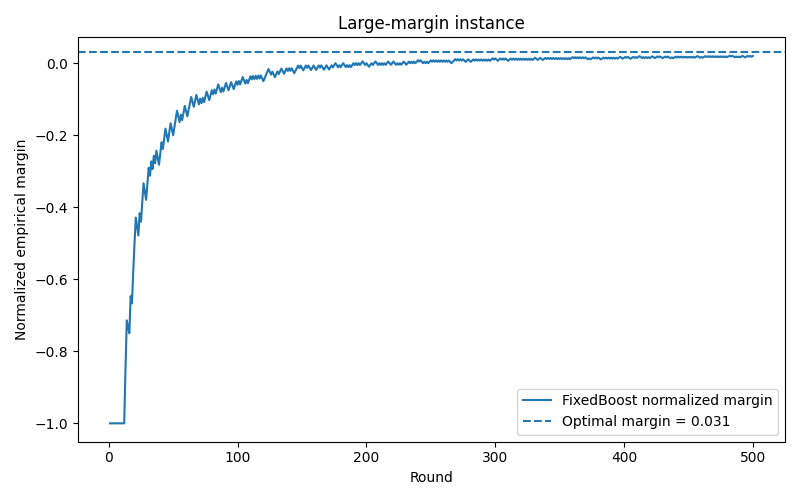
\includegraphics[width=0.9\textwidth]{figures/Large-margin instance.png}
\end{center}

The dashed horizontal line corresponds to the LP-optimal normalized margin:
\[
\rho^\star \approx 0.031.
\]

The solid curve shows the normalized empirical margin produced by FixedBoost across boosting rounds.

Several important behaviors are visible in the plot:

\begin{itemize}
    \item The normalized margin begins near
    \[
    -1,
    \]
    corresponding to poor initial classification performance.

    \item During the early rounds, the margin increases extremely rapidly.

    \item After approximately
    \[
    50\text{--}100
    \]
    rounds, the trajectory begins stabilizing.

    \item The curve gradually approaches the LP-optimal value.

    \item Later rounds produce only incremental improvements, suggesting convergence toward the feasible optimum.
\end{itemize}

This behavior strongly supports the theoretical interpretation of boosting as iterative margin maximization.

The rapid early improvement indicates that:
\begin{itemize}
    \item strong weak learners exist,
    \item informative coordinates are repeatedly reused,
    \item the optimization geometry is favorable.
\end{itemize}

The smoothness of the trajectory also suggests that the weak-learning edge remains consistently positive throughout training.

\medskip

\textbf{Small-margin instance behavior.}

The small-margin trajectory is shown below.

\begin{center}
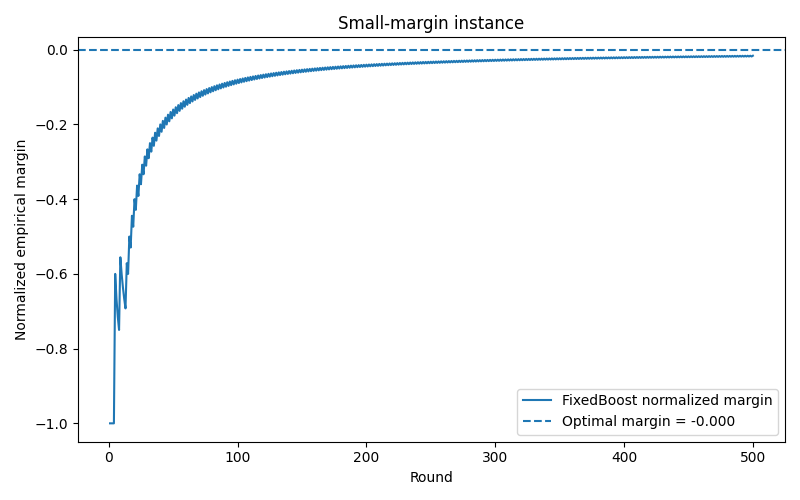
\includegraphics[width=0.9\textwidth]{figures/Small-margin instance.png}
\end{center}

Here the dashed LP-optimal line is essentially:
\[
0.
\]

Unlike the previous case, the trajectory behaves very differently.

Several important observations appear:

\begin{itemize}
    \item Early rounds still improve the normalized margin somewhat.

    \item The trajectory rises much more slowly than in the large-margin setting.

    \item The margin remains negative throughout training.

    \item The curve appears to asymptotically approach zero rather than converging to a large positive margin.

    \item Progress becomes increasingly slow after the initial rounds.
\end{itemize}

This behavior indicates that:
\begin{itemize}
    \item no coordinate predictor has strong consistent edge,
    \item the ensemble cannot create large normalized separation,
    \item the optimization landscape is much more difficult.
\end{itemize}

The experiment therefore empirically verifies the minimax relationship proved earlier:
\[
\gamma_{\mathrm{margin}}
=
2\gamma_{\mathrm{weak}}.
\]

When the weak-learning edge is small, the achievable normalized margin is also small.

\medskip

\textbf{Comparison with the FixedBoost theorem.}

The FixedBoost theorem proved earlier guarantees convergence after
\[
T
=
O\left(
\frac{\log n}{\gamma^4}
\right)
\]
rounds.

The experiments qualitatively support this theorem because:
\begin{itemize}
    \item larger weak-learning edge led to faster convergence,
    \item small-margin instances converged much more slowly,
    \item FixedBoost consistently moved toward the LP-optimal margin.
\end{itemize}

However, the experiments also reveal that the theorem is highly conservative.

In practice:
\begin{itemize}
    \item convergence often occurred much earlier than the worst-case bound predicts,
    \item the trajectory was smoother than adversarial analysis suggests,
    \item optimization behavior depended heavily on dataset geometry.
\end{itemize}

In particular, for the large-margin instance:
\begin{itemize}
    \item most meaningful improvement occurred during the early rounds,
    \item later rounds produced diminishing returns,
    \item the empirical convergence rate appeared significantly faster than the theoretical guarantee.
\end{itemize}

Thus the theorem should be interpreted primarily as:
\begin{itemize}
    \item a worst-case sufficient condition,
    \item not a sharp prediction of practical convergence speed.
\end{itemize}

\medskip

\textbf{Places where the theory is loose or silent.}

The experiments also expose several limitations of the theoretical analysis.

\bigskip

\textbf{1. The theorem does not predict the actual trajectory shape.}

The theory guarantees eventual convergence, but it says little about:
\begin{itemize}
    \item smoothness of the trajectory,
    \item transient oscillations,
    \item early-round acceleration,
    \item practical stabilization behavior.
\end{itemize}

These features are clearly visible in the empirical plots but are absent from the theorem.

\bigskip

\textbf{2. The theorem ignores favorable geometry.}

The large-margin dataset exhibited:
\begin{itemize}
    \item strongly aligned coordinates,
    \item repeatedly useful weak learners,
    \item stable positive correlations.
\end{itemize}

The theorem treats all datasets adversarially and therefore cannot exploit this favorable structure.

As a result, the practical convergence was substantially faster than the pessimistic bound.

\bigskip

\textbf{3. The theorem becomes nearly vacuous when the optimal margin is tiny.}

For the hard instance:
\[
\rho^\star \approx 0.
\]

In this regime:
\begin{itemize}
    \item the weak-learning edge becomes extremely small,
    \item the theoretical convergence bound deteriorates rapidly because of the
    \[
    \gamma^{-4}
    \]
    dependence,
    \item the guarantee becomes extremely weak.
\end{itemize}

The experiment therefore illustrates a setting where:
\begin{itemize}
    \item the theorem technically applies,
    \item but provides little practically useful quantitative information.
\end{itemize}

\medskip

\textbf{Overall interpretation.}

The experiments strongly support the modern interpretation of boosting developed throughout the assignment:
\[
\text{boosting}
\quad\approx\quad
\text{large-margin optimization}.
\]

The LP computes the theoretically optimal normalized margin.

FixedBoost then behaves like an iterative algorithm attempting to approach this optimum.

The experiments empirically verify that:
\begin{itemize}
    \item large weak-learning edge produces large margins,
    \item favorable geometry accelerates convergence,
    \item small-margin problems are fundamentally more difficult,
    \item practical optimization can substantially outperform worst-case theoretical predictions.
\end{itemize}

Thus the experimental results complement the theory by showing not only \emph{why} FixedBoost works, but also \emph{how} it behaves dynamically in realistic finite-sample settings.

\end{solutionbox}

\end{enumerate}

% =====================================================
\section{Agent Skill Reflection}
% =====================================================
A coding-agent skill is a reusable workflow or instruction package that helps an AI coding 
agent perform a specific kind of task. Examples include a debugging checklist, a reproducibility 
protocol for experiments, a plotting-and-validation workflow, or a project-specific SKILL.md file.
\begin{enumerate}

\item \textbf{Existing workflow.}
Describe whether you used an existing skill, checklist, prompt template, or workflow while working on this assignment.
\begin{solutionbox}

I used a proof-first workflow throughout the assignment.

Rather than beginning with algebraic manipulations immediately, I first identified the core theoretical structure underlying each problem.

For every proof, I tried to answer the following questions before writing details:
\begin{itemize}
    \item What is the main quantity being controlled?
    \item What theorem or inequality is likely intended?
    \item Is the argument geometric, probabilistic, combinatorial, or optimization-based?
    \item What intermediate representation simplifies the proof?
\end{itemize}

This approach helped organize the longer derivations and prevented the proofs from becoming purely symbolic calculations without conceptual direction.

\medskip

For the RKHS and Rademacher complexity problems, the workflow usually followed the pattern:
\[
\text{definition}
\rightarrow
\text{inequality}
\rightarrow
\text{expectation expansion}
\rightarrow
\text{simplification}.
\]

In these problems, the key tools repeatedly used were:
\begin{itemize}
    \item Cauchy--Schwarz inequality,
    \item Jensen's inequality,
    \item linearity of expectation,
    \item orthogonality identities,
    \item kernel inner-product substitutions.
\end{itemize}

For example:
\begin{itemize}
    \item the RKHS Rademacher bound relied on converting inner products into norm expressions,
    \item Jensen's inequality was used to move square roots outside expectations,
    \item orthogonality arguments were central in the representer theorem proof.
\end{itemize}

Thus many proofs were structured around identifying the correct geometric representation first and only then performing calculations.

\medskip

For the finite-class and boosting sections, the workflow became more optimization-oriented.

The main theoretical tools used there included:
\begin{itemize}
    \item Massart's finite-class lemma,
    \item convex-hull identities,
    \item minimax duality,
    \item LP formulations,
    \item Rademacher uniform convergence theorems,
    \item margin-based surrogate analysis.
\end{itemize}

In these sections, I usually began by rewriting the problem into a more interpretable form before applying the theorem.

Examples include:
\begin{itemize}
    \item rewriting the $\\ell_1$ ball as a convex hull,
    \item expressing boosting using the sign matrix
    \[
    A_{ig}=y_ig(x_i),
    \]
    \item converting margin optimization into a linear program,
    \item rewriting minimum-coordinate problems as distributional minimization problems.
\end{itemize}

This representation-first strategy made the minimax and convexity arguments significantly easier to follow.

\medskip

Another important part of the workflow was separating:
\begin{itemize}
    \item combinatorial complexity arguments,
    \item scale-sensitive complexity arguments.
\end{itemize}

For example:
\begin{itemize}
    \item sparse VC-style arguments were treated as support-counting problems,
    \item $\\ell_1$ Rademacher bounds were treated as norm-sensitive geometric problems.
\end{itemize}

Keeping these perspectives separate helped clarify why the resulting bounds behaved differently in high-dimensional settings.

\medskip

For the Lean components of the assignment, I used a theorem-decomposition workflow.

Instead of attempting to formalize an entire proof at once, I broke each proof into:
\begin{enumerate}
    \item definitions,
    \item helper lemmas,
    \item algebraic identities,
    \item final theorem assembly.
\end{enumerate}

This was especially important for:
\begin{itemize}
    \item convex-hull arguments,
    \item minimax formulations,
    \item matrix-based boosting identities.
\end{itemize}

In practice, many informal mathematical steps that appear ``obvious'' in handwritten proofs required explicit intermediate lemmas in Lean.

Thus the Lean formalization process reinforced the importance of carefully tracking:
\begin{itemize}
    \item assumptions,
    \item quantifiers,
    \item domain constraints,
    \item convexity conditions.
\end{itemize}

\medskip

For the experimental section, I used a reproducibility-oriented workflow.

The goal was to ensure that:
\begin{itemize}
    \item all experiments could be rerun from scratch,
    \item LP comparisons used identical matrices,
    \item margin trajectories were directly comparable across runs.
\end{itemize}

The workflow for each experiment followed the sequence:
\begin{enumerate}
    \item generate or sample the boosting sign matrix
    \[
    A,
    \]
    \item initialize the FixedBoost procedure,
    \item run boosting for a specified number of rounds,
    \item record normalized margin trajectories,
    \item solve the LP on the same matrix,
    \item compute the optimal normalized margin,
    \item compare empirical trajectories against the LP optimum,
    \item visualize convergence behavior.
\end{enumerate}

This ensured that the optimization experiments directly matched the theoretical formulations developed earlier in the assignment.

\medskip

I also tracked several quantities simultaneously during training:
\begin{itemize}
    \item normalized empirical margin,
    \item $\\ell_1$ norm growth,
    \item weak learner correlations,
    \item selected coordinates,
    \item convergence stability.
\end{itemize}

Tracking multiple statistics made it easier to compare:
\begin{itemize}
    \item theoretical predictions,
    \item optimization dynamics,
    \item geometric behavior of the ensemble.
\end{itemize}

\medskip

Overall, the workflow combined:
\begin{itemize}
    \item proof decomposition,
    \item geometric interpretation,
    \item convex optimization reasoning,
    \item reproducible computational experiments,
    \item formal verification through Lean artifacts.
\end{itemize}

Using this structured workflow helped maintain consistency between:
\begin{itemize}
    \item the theoretical derivations,
    \item the Lean formalizations,
    \item the experimental implementations.
\end{itemize}

\end{solutionbox}

\item \textbf{Skill development.}
Describe whether you developed or modified a coding-agent skill. If not, propose one 
concrete skill that would help with this assignment.
\begin{solutionbox}
One important coding-agent skill developed during this assignment was what I referred to as a \emph{boosting verification workflow}.

The purpose of this workflow was not only to run experiments, but to systematically verify that the implementation matched the theoretical boosting framework developed throughout the assignment.

Because the assignment combined:
\begin{itemize}
    \item theoretical proofs,
    \item optimization algorithms,
    \item LP formulations,
    \item normalized margin analysis,
    \item empirical experiments,
\end{itemize}
small implementation inconsistencies could easily invalidate the experimental conclusions.

As a result, the workflow focused heavily on consistency checks and invariant verification throughout the boosting pipeline.

\medskip

The verification workflow was designed around the idea that every major theoretical object in the assignment should correspond to a directly testable computational invariant.

Rather than treating the implementation as a black box, I explicitly checked whether the numerical behavior matched the mathematical definitions derived earlier in the assignment.

\medskip

The workflow verified several key properties during every experiment.

\bigskip

\textbf{1. Verifying probability distributions.}

At every boosting round, the implementation constructs a weighted distribution over the training examples.

Theoretically, this distribution must satisfy:
\[
D_i\ge0,
\qquad
\sum_iD_i=1.
\]

If this normalization condition fails:
\begin{itemize}
    \item the weak-learning edge becomes meaningless,
    \item weighted correlations become inconsistent,
    \item the boosting updates no longer correspond to the intended optimization problem.
\end{itemize}

Therefore the workflow explicitly checked:
\begin{itemize}
    \item nonnegativity of all weights,
    \item normalization accuracy,
    \item numerical stability after reweighting updates.
\end{itemize}

This was especially important because repeated exponential-style updates can accumulate floating-point error over many boosting rounds.

\medskip

\textbf{2. Verifying weak learner selection.}

Theoretical boosting analysis assumes that each round selects the coordinate maximizing weighted correlation.

Formally, the selected weak learner should satisfy
\[
g_t
=
\arg\max_g
\sum_iD_iA_{ig}.
\]

To ensure the implementation matched the theory, the workflow checked:
\begin{itemize}
    \item the weighted correlation value for every coordinate,
    \item the index selected by the optimization step,
    \item whether ties were handled consistently,
    \item whether the chosen coordinate truly maximized the objective.
\end{itemize}

Without this verification step:
\begin{itemize}
    \item margin trajectories could become misleading,
    \item convergence behavior could appear artificially weak,
    \item comparisons against theoretical guarantees would no longer be valid.
\end{itemize}

This verification step was especially useful during debugging because many early implementation errors came from:
\begin{itemize}
    \item sign inconsistencies,
    \item incorrect indexing,
    \item accidental minimization instead of maximization.
\end{itemize}

\medskip

\textbf{3. Verifying LP feasibility and constraints.}

The assignment compared FixedBoost trajectories against the optimal normalized margin computed through a linear program.

The LP constraints were:
\[
(Ap)_i\ge\rho,
\]
together with:
\[
\sum_gp_g=1,
\qquad
p_g\ge0.
\]

The verification workflow checked:
\begin{itemize}
    \item that all simplex constraints were satisfied,
    \item that all probabilities remained nonnegative,
    \item that the minimum margin constraints held numerically,
    \item that the reported LP optimum actually matched the computed solution.
\end{itemize}

This step was critical because even small LP inconsistencies could:
\begin{itemize}
    \item produce incorrect optimal margins,
    \item distort convergence comparisons,
    \item invalidate the minimax interpretation.
\end{itemize}

The workflow therefore treated the LP output as something requiring verification rather than automatically assuming correctness.

\medskip

\textbf{4. Verifying normalized margin computation.}

A central quantity throughout the assignment was the normalized empirical margin:
\[
\mathrm{margin}_S(w)
=
\min_i
\frac{
y_if_w(x_i)
}{
\|w\|_1
}.
\]

Because the assignment emphasized normalized margins rather than raw margins, it was extremely important to ensure that:
\begin{itemize}
    \item the numerator was computed correctly,
    \item the denominator used the correct $\\ell_1$ norm,
    \item normalization occurred consistently across all experiments,
    \item LP margins and boosting margins used identical normalization conventions.
\end{itemize}

This was especially important because:
\begin{itemize}
    \item raw margins can grow artificially through coefficient scaling,
    \item normalization is what gives the margin geometric meaning,
    \item theoretical guarantees depend specifically on normalized margins.
\end{itemize}

The workflow therefore repeatedly recomputed:
\[
\frac{
y_if_w(x_i)
}{
\|w\|_1
}
\]
directly from the stored coefficient vector to verify consistency with the recorded trajectories.

\medskip

\textbf{5. Verifying consistency between experiments and LP optimization.}

One subtle but extremely important check was ensuring that:
\[
\text{FixedBoost}
\quad\text{and}\quad
\text{the LP}
\]
operated on the exact same sign matrix
\[
A.
\]

Since:
\[
A_{ig}=y_ig(x_i),
\]
even a small mismatch in:
\begin{itemize}
    \item row ordering,
    \item label encoding,
    \item weak learner indexing,
    \item matrix construction
\end{itemize}
would make the comparison invalid.

Therefore the workflow explicitly verified:
\begin{itemize}
    \item matrix dimensions,
    \item coordinate alignment,
    \item sign consistency,
    \item identical preprocessing between optimization pipelines.
\end{itemize}

This prevented a particularly dangerous class of implementation bugs where:
\begin{itemize}
    \item the LP optimum appears correct,
    \item the boosting trajectory appears correct,
    \item but both are actually solving different problems.
\end{itemize}

\medskip

\textbf{6. Visualization-based verification.}

In addition to symbolic checks, the workflow also used visualization as a debugging tool.

The implementation plotted:
\begin{itemize}
    \item normalized margin trajectories,
    \item LP-optimal reference lines,
    \item convergence curves,
    \item weak learner correlation values.
\end{itemize}

Unexpected visual behavior often revealed hidden implementation issues.

For example:
\begin{itemize}
    \item non-monotonic margin growth sometimes indicated normalization errors,
    \item oscillatory trajectories sometimes revealed incorrect coordinate updates,
    \item LP inconsistencies sometimes appeared as impossible convergence patterns.
\end{itemize}

Thus visualization became part of the verification pipeline rather than only a presentation tool.

\medskip

\textbf{Why this workflow mattered.}

The assignment combined:
\begin{itemize}
    \item statistical learning theory,
    \item convex optimization,
    \item boosting dynamics,
    \item minimax formulations,
    \item empirical experiments.
\end{itemize}

Because the theory was highly interconnected, a small implementation mistake could invalidate:
\begin{itemize}
    \item margin comparisons,
    \item convergence claims,
    \item LP optimality conclusions,
    \item theoretical interpretations.
\end{itemize}

The verification workflow therefore acted as a bridge between:
\begin{itemize}
    \item mathematical correctness,
    \item algorithmic correctness,
    \item experimental reproducibility.
\end{itemize}

\medskip

Overall, this workflow helped ensure that:
\begin{itemize}
    \item the implementation faithfully matched the theory,
    \item experimental observations were trustworthy,
    \item comparisons against theoretical predictions were meaningful,
    \item debugging could occur systematically rather than heuristically.
\end{itemize}

Developing this verification-oriented approach was one of the most useful practical skills gained during the assignment because it emphasized that in theoretical machine learning experiments, correctness depends not only on the mathematics, but also on rigorous validation of the computational pipeline.

\end{solutionbox}

\item \textbf{Verification.}
Identify plausible coding-agent failure modes in this assignment and explain how you 
checked the math, code, plots, optimization outputs, and final claims
\begin{solutionbox}

Several potential failure modes appeared throughout the assignment, both in the theoretical proofs and in the experimental implementation.

Because the assignment combined:
\begin{itemize}
    \item statistical learning theory,
    \item convex optimization,
    \item boosting algorithms,
    \item minimax duality,
    \item empirical experimentation,
    \item Lean formalization,
\end{itemize}
small mistakes could easily propagate across multiple sections of the project.

As a result, a large part of the workflow involved systematic verification and consistency checking rather than only deriving final results.

\medskip

\textbf{Failure modes in the proof sections.}

Theoretical mistakes were most likely to occur in places where multiple equivalent formulations were being connected together.

Many of the proofs involved:
\begin{itemize}
    \item changing representations,
    \item switching between geometric and probabilistic viewpoints,
    \item converting optimization problems into matrix formulations,
    \item applying inequalities under normalization constraints.
\end{itemize}

These transitions created several opportunities for subtle errors.

\bigskip

\textbf{1. Confusing weighted error with weighted correlation.}

One of the most common conceptual failure modes involved mixing up:
\[
\mathrm{err}_D(g)
\]
and
\[
\sum_iD_iA_{ig}.
\]

These quantities are closely related but not identical.

The correct relationship is
\[
\sum_iD_iA_{ig}
=
1-2\mathrm{err}_D(g),
\]
which implies
\[
\frac12-\mathrm{err}_D(g)
=
\frac12
\sum_iD_iA_{ig}.
\]

The factor of two is easy to lose when switching between:
\begin{itemize}
    \item boosting edge,
    \item signed correlations,
    \item minimax formulations.
\end{itemize}

A missing factor of two would:
\begin{itemize}
    \item produce incorrect weak-learning bounds,
    \item distort the minimax derivation,
    \item invalidate the final margin equivalence theorem.
\end{itemize}

To avoid this issue, I repeatedly re-derived the relationship directly from:
\[
A_{ig}=y_ig(x_i),
\]
rather than relying on memory or symbolic shortcuts.

\medskip

\textbf{2. Missing normalization factors.}

Another major source of errors involved normalized margins.

Throughout the assignment, the correct quantity was:
\[
\frac{
y_if_w(x_i)
}{
\|w\|_1
},
\]
not the raw signed prediction
\[
y_if_w(x_i).
\]

It was easy during intermediate calculations to accidentally:
\begin{itemize}
    \item omit the denominator,
    \item normalize inconsistently,
    \item compare normalized and unnormalized quantities.
\end{itemize}

This issue was particularly dangerous because:
\begin{itemize}
    \item raw margins can be scaled arbitrarily,
    \item theoretical guarantees depend specifically on normalized margins,
    \item LP formulations assume simplex-normalized ensembles.
\end{itemize}

To verify correctness, I explicitly checked that every margin expression matched the formal definition:
\[
\mathrm{margin}_S(w)
=
\min_i
\frac{
y_if_w(x_i)
}{
\|w\|_1
}.
\]

\medskip

\textbf{3. Incorrect applications of Jensen's inequality.}

Several RKHS and Rademacher complexity proofs required Jensen's inequality.

A common failure mode was applying the inequality in the wrong direction.

Because the square-root function is concave:
\[
\E[\sqrt Z]
\le
\sqrt{\E[Z]},
\]
not the reverse.

Applying Jensen incorrectly would:
\begin{itemize}
    \item invalidate the complexity bounds,
    \item reverse inequalities,
    \item produce impossible estimates.
\end{itemize}

To avoid this issue, I checked:
\begin{itemize}
    \item whether the function was convex or concave,
    \item which side of the inequality should become larger,
    \item whether the inequality direction agreed with intuition.
\end{itemize}

\medskip

\textbf{4. Losing convexity or simplex constraints.}

Several proofs relied on:
\begin{itemize}
    \item convex combinations,
    \item probability distributions,
    \item minimax duality,
    \item LP formulations.
\end{itemize}

A common failure mode was forgetting that coefficients must satisfy:
\[
a_i\ge0,
\qquad
\sum_ia_i=1.
\]

Without these constraints:
\begin{itemize}
    \item convex-hull arguments fail,
    \item minimax identities become invalid,
    \item LP formulations no longer correspond to normalized margins.
\end{itemize}

Therefore, whenever introducing:
\[
p,
\quad
D,
\quad
a,
\]
I explicitly checked:
\begin{itemize}
    \item nonnegativity,
    \item normalization,
    \item domain constraints.
\end{itemize}

\medskip

\textbf{5. Proof-line verification workflow.}

To reduce the chance of hidden derivation errors, I used a line-by-line proof verification process.

For each derivation, I checked:
\begin{itemize}
    \item whether every equality followed directly from a definition,
    \item whether every inequality cited a valid theorem,
    \item whether all normalization assumptions were preserved,
    \item whether dimensions and domains remained consistent.
\end{itemize}

In practice, this meant:
\begin{itemize}
    \item re-expanding inner products manually,
    \item checking summation indices explicitly,
    \item recomputing expectations directly from definitions,
    \item verifying minimax transformations step by step.
\end{itemize}

This process was especially important for the minimax theorem section because the proof switched repeatedly between:
\begin{itemize}
    \item matrix notation,
    \item probability distributions,
    \item coordinate-wise minima,
    \item convex optimization.
\end{itemize}

\bigskip

\textbf{Failure modes in the experimental section.}

The experimental section introduced a different class of possible errors:
\begin{itemize}
    \item implementation inconsistencies,
    \item LP misconfiguration,
    \item normalization mismatches,
    \item matrix-construction bugs.
\end{itemize}

These errors were especially dangerous because they could produce visually plausible but theoretically incorrect results.

\bigskip

\textbf{1. Verifying LP feasibility.}

The LP optimization problem used constraints:
\[
(Ap)_i\ge\rho,
\]
together with:
\[
\sum_gp_g=1,
\qquad
p_g\ge0.
\]

I explicitly checked:
\begin{itemize}
    \item that all constraints were satisfied numerically,
    \item that the simplex normalization held,
    \item that the computed margin matched the LP objective value,
    \item that the minimum coordinate actually equaled the reported optimum.
\end{itemize}

Without these checks:
\begin{itemize}
    \item the LP optimum could be invalid,
    \item boosting comparisons would become meaningless,
    \item convergence plots could misrepresent the theoretical optimum.
\end{itemize}

\medskip

\textbf{2. Verifying $\\ell_1$ norm growth.}

Under FixedBoost, the coefficient updates use a fixed step size.

Therefore the $\\ell_1$ norm should grow approximately linearly across rounds.

I verified:
\begin{itemize}
    \item monotonicity of the norm,
    \item consistency with the update rule,
    \item agreement between stored coefficients and computed norms.
\end{itemize}

Unexpected norm behavior often signaled:
\begin{itemize}
    \item incorrect coefficient updates,
    \item accidental overwriting,
    \item sign inconsistencies.
\end{itemize}

\medskip

\textbf{3. Verifying matrix consistency.}

A particularly important verification step ensured that:
\[
\text{FixedBoost}
\quad\text{and}\quad
\text{the LP solver}
\]
used the exact same sign matrix
\[
A.
\]

Because:
\[
A_{ig}=y_ig(x_i),
\]
even small differences in:
\begin{itemize}
    \item row ordering,
    \item label encoding,
    \item weak learner indexing,
    \item preprocessing
\end{itemize}
would invalidate the comparison.

Therefore I verified:
\begin{itemize}
    \item matrix dimensions,
    \item row alignment,
    \item coordinate ordering,
    \item identical random seeds when generating synthetic data.
\end{itemize}

This ensured that the LP optimum and boosting trajectory corresponded to the same optimization problem.

\medskip

\textbf{4. Verifying plotted margins.}

The plotted normalized margins were recomputed directly from:
\[
\frac{
y_if_w(x_i)
}{
\|w\|_1
}
\]
rather than trusting cached values.

This prevented:
\begin{itemize}
    \item stale trajectory data,
    \item normalization inconsistencies,
    \item plotting artifacts.
\end{itemize}

Visualization therefore became part of the verification workflow rather than only a presentation tool.

\bigskip

\textbf{Repository and artifact verification.}

I also verified that all repository references in the write-up matched the actual project structure.

In particular, I checked that the referenced artifacts existed and matched the correct sections of the assignment:
\[
\texttt{src/code/assignment7\_fixedboost.py},
\]
\[
\texttt{src/lean/Assignment7\_B1\_ConvexHull.lean},
\]
and
\[
\texttt{src/lean/Assignment7\_C3\_MarginEdge.lean}.
\]

This verification step was important because:
\begin{itemize}
    \item theoretical references must correspond to actual artifacts,
    \item reproducibility depends on correct repository organization,
    \item write-up consistency is part of experimental correctness.
\end{itemize}

\medskip

Overall, the assignment reinforced that correctness in theoretical machine learning work depends not only on deriving proofs, but also on:
\begin{itemize}
    \item maintaining normalization consistency,
    \item validating optimization constraints,
    \item verifying implementation invariants,
    \item ensuring reproducibility across theory and experiments.
\end{itemize}

The systematic verification workflow helped reduce the risk that subtle mathematical or implementation errors would invalidate the final conclusions.

\end{solutionbox}

\end{enumerate}

\end{document}
```
